\documentclass[a4paper,12pt]{article}

%%% Работа с русским языком
\usepackage{cmap}					% поиск в PDF
% \usepackage{mathtext} 				% русские буквы в формулах
\usepackage[T2A]{fontenc}			% кодировка
\usepackage[utf8]{inputenc}			% кодировка исходного текста
\usepackage[english,russian]{babel}	% локализация и переносы

%%% Страница
\usepackage{extsizes} % Возможность сделать 14-й шрифт
\usepackage{geometry} % Создание полей
\usepackage{indentfirst} % Пакет для установки красной строки для первого абзаца в разделе
\geometry{top = 2.5cm}
\geometry{bottom = 2cm}
\geometry{left = 3cm}
\geometry{right = 1.5cm}
\renewcommand{\baselinestretch}{1.5} % Интерлиньяж 1.5

%%% Дополнительная работа с математикой
\usepackage{amsmath,amsfonts,amssymb,amsthm,mathtools} % AMS
\usepackage{icomma} % "Умная" запятая: $0,2$ --- число, $0, 2$ --- перечисление

%% Номера формул
%\mathtoolsset{showonlyrefs=true} % Показывать номера только у тех формул, на которые есть \eqref{} в тексте.
%\usepackage{leqno} % Нумерация формул слева

%% Свои команды
\DeclareMathOperator{\sgn}{\mathop{sgn}}

%% Перенос знаков в формулах (по Львовскому)
\newcommand*{\hm}[1]{#1\nobreak\discretionary{}
	{\hbox{$\mathsurround=0pt #1$}}{}}

%%% Работа с картинками
\usepackage{graphicx}  % Для вставки рисунков
\graphicspath{{images/}{images2/}}  % папки с картинками
\setlength\fboxsep{3pt} % Отступ рамки \fbox{} от рисунка
\setlength\fboxrule{1pt} % Толщина линий рамки \fbox{}
\usepackage{wrapfig} % Обтекание рисунков текстом

%%% Работа с таблицами
\usepackage{array,tabularx,tabulary,booktabs} % Дополнительная работа с таблицами
\usepackage{longtable}  % Длинные таблицы
\usepackage{multirow} % Слияние строк в таблице

%%% Теоремы
\theoremstyle{plain} % Стиль по умолчанию
\newtheorem{theorem}{Теорема}[section]
\newtheorem{proposition}[theorem]{Утверждение}

\theoremstyle{definition} % "Определение"
\newtheorem{corollary}{Следствие}[theorem]
\newtheorem{problem}{Задача}[section]

\theoremstyle{remark} % "Примечание"
\newtheorem*{nonum}{Решение}

%%% Программирование
\usepackage{etoolbox} % логические операторы

\usepackage{lastpage} % Узнать, сколько всего страниц в документе.

\usepackage{soul} % Модификаторы начертания

\usepackage{graphicx} %Подключаю модули для добавления картинок
\graphicspath{.}
\DeclareGraphicsExtensions{.pdf,.png,.jpg}
	
	\renewcommand{\baselinestretch}{1.5}
	
\begin{document}
\renewcommand{\contentsname}{\Large Содержание}
\renewcommand{\bibname}{\normalfont\Large\bfseries Список литературы}

\begin{titlepage}
	\begin{center}
		Министерство науки и высшего образования Российской Федерации \\
		НАЦИОНАЛЬНЫЙ ИССЛЕДОВАТЕЛЬСКИЙ ЯДЕРНЫЙ УНИВЕРСИТЕТ <<МИФИ>> \\*
		\hrulefill
	\end{center}
	
	\begin{center}
		ИНСТИТУТ ЛАЗЕРНЫХ И ПЛАЗМЕННЫХ ТЕХНОЛОГИЙ\\
		КАФЕДРА №31 ПРИКЛАДНАЯ МАТЕМАТИКА
	\end{center}
	\vspace{1cm}
	
	\vspace{2em}
	
	\begin{center}
		\large{Отчет}
		
		по научно-исследовательской работе на тему:
	\end{center}
	\begin{center}
		\large <<Оптимизация канального радиатора>>
	\end{center}
	\begin{center}
		\large \textit{Выполнил: Есис А. И.}
		
		\textit{Руководитель проекта: Чмыхов М. А.}
	\end{center}
	
	
	\vspace{22em}
	
	\begin{center}
		г. Москва 2023
	\end{center}
\end{titlepage}

\newpage
\section*{Аннотация}

В данной работе проведено комплексное исследование теплоотводящей системы радиатора с использованием интегрированных вычислительных инструментов. В начальной стадии исследования была построена геометрия и сетка радиатора с применением программного комплекса SALOME Meca. Далее, для получения данных о тепловом и газодинамическом поведении системы, были проведены численные симуляции с использованием программного пакета OpenFOAM.

Основным этапом работы стал анализ результатов численных симуляций и СОВЕРШЕНСТВОВАНИЯ геометрии радиатора с использованием методов оптимизации. Первоначальная оптимизация включала в себя полный перебор точек в пространстве параметров, что позволило выделить оптимальные конфигурации. ЗАТЕМ был применен эволюционный алгоритм, который существенно ускорил процесс оптимизации, сократив количество необходимых расчетов.

Дополнительно, использовались градиентные методы оптимизации, такие как L-BFGS-B, для повышения эффективности процесса оптимизации. Каждый этап исследования включал в себя визуализацию результатов при помощи ParaView.

Полученные результаты могут быть использованы для разработки и улучшения радиаторов в различных инженерных областях, где теплоотвод играет ключевую роль.

\newpage 
\tableofcontents
\setcounter{page}{3}

\newpage
\section{Введение}


\section{Введение}

Программные продукты OpenFOAM, ParaView и SALOME Meca представляют собой мощный инструментарий, широко используемый в области вычислительной гидрогазодинамики (CFD) и численного моделирования. Совместное использование этих инструментов обеспечивает комплексное решение для анализа и визуализации сложных физических процессов, таких как течение жидкостей, теплообмен, движение твердых тел и другие.

OpenFOAM (Open Field Operation and Manipulation) -- свободное и открытое программное обеспечение, предназначенное для решения уравнений Навье-Стокса и других математических моделей, связанных с течением жидкостей и газов. Этот инструмент предоставляет разнообразные методы решения, что позволяет исследовать различные типы потоков и применять различные физические модели. OpenFOAM является расширяемым и настраиваемым инструментом, который можно адаптировать под конкретные задачи и требования.

ParaView обеспечивает возможности визуализации результатов численных симуляций. Он поддерживает создание различных графических представлений, включая 2D и 3D графику, контурные изображения, срезы и анимации. ParaView также обладает интерактивными возможностями для анализа данных в реальном времени и взаимодействия с моделью, что облегчает глубокий анализ результатов.

SALOME Meca является интегрированной средой для предварительной обработки геометрии и настройки расчетной сетки для OpenFOAM. Этот инструмент обеспечивает интуитивный пользовательский интерфейс для создания и манипулирования сложными геометрическими моделями, а также настройки сеток различной структуры. SALOME Meca предоставляет инструменты для проверки качества сетки и ее подготовки к последующим симуляциям в OpenFOAM \cite{wOfDocSalome}.

В совокупности OpenFOAM, ParaView и SALOME Meca предоставляют мощный комплект инструментов для моделирования и визуализации в области CFD. Они позволяют проводить сложные численные симуляции, анализировать результаты и визуализировать данные, способствуя лучшему пониманию физических процессов и принятию информированных решений в различных областях применения, таких как авиация, автомобильная промышленность, энергетика и др.

\newpage
\section{Данные предыдущего этапа исследования}

В данном проекте исследуется задача охлаждения нагретого тела с помощью установки радиатора.

В начале проекта геометрия радиатора строится с использованием графического интерфейса SALOME. Используя интуитивно понятный пользовательский интерфейс, создается геометрия радиатора. Этот этап позволяет получить исходную геометрию, которая будет использоваться для последующих анализов.

Затем, для повышения гибкости и автоматизации процесса, создается скрипт на языке Python, который генерирует геометрию радиатора. В этом скрипте можно устанавливать параметры радиатора, такие как расположение элементов. Это позволяет быстро создавать и изменять различные варианты геометрии радиатора для дальнейшего анализа и оптимизации.

Для исследования были использованы три различных варианта геометрии радиатора.
Примеры геометрии:
\begin{figure}[h]
	\begin{center}
		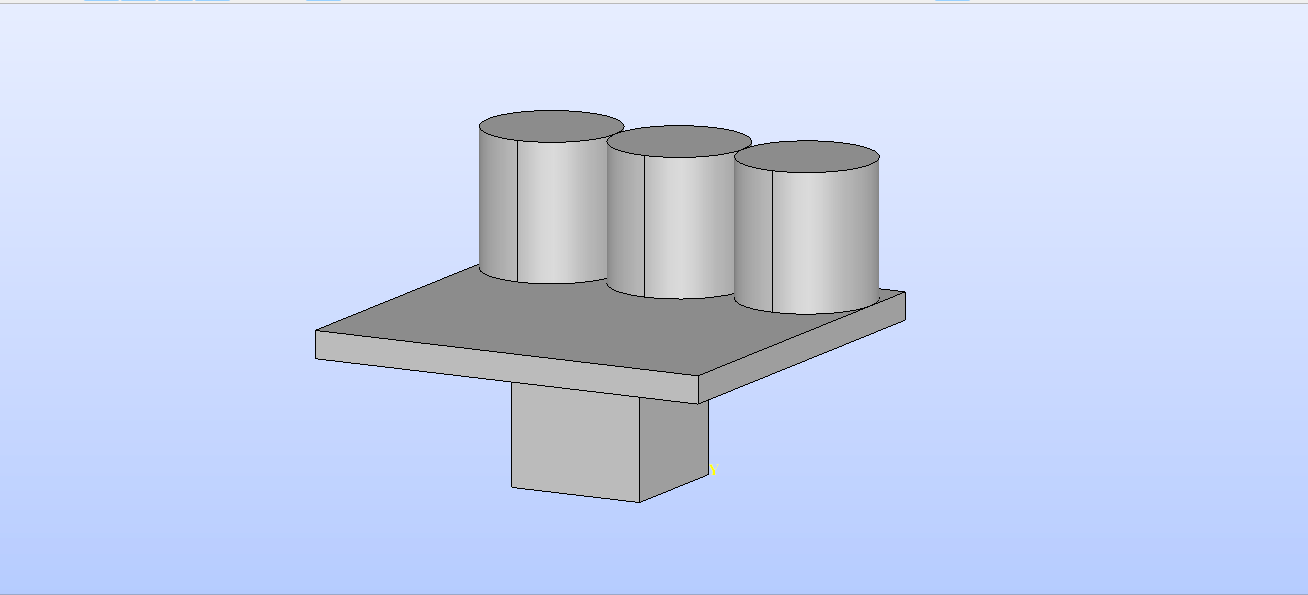
\includegraphics[width=0.5\linewidth]{1.1.png}
		\caption{Модель геометрии 1} %% подпись к рисунку
	\end{center}
\end{figure}
\begin{figure}[h]
	\begin{center}
		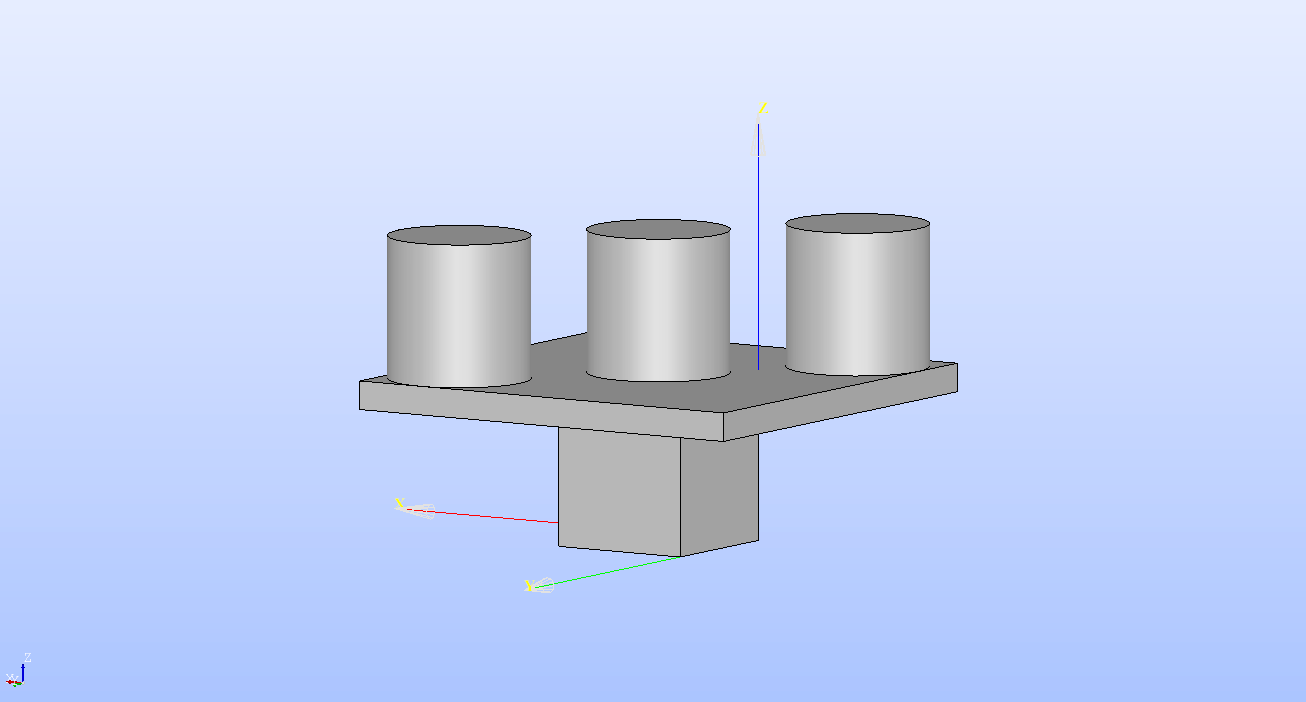
\includegraphics[width=0.5\linewidth]{1.2.png}
		\caption{Модель геометрии 2}
	\end{center}
\end{figure}
\begin{figure}[h]
	\begin{center}
		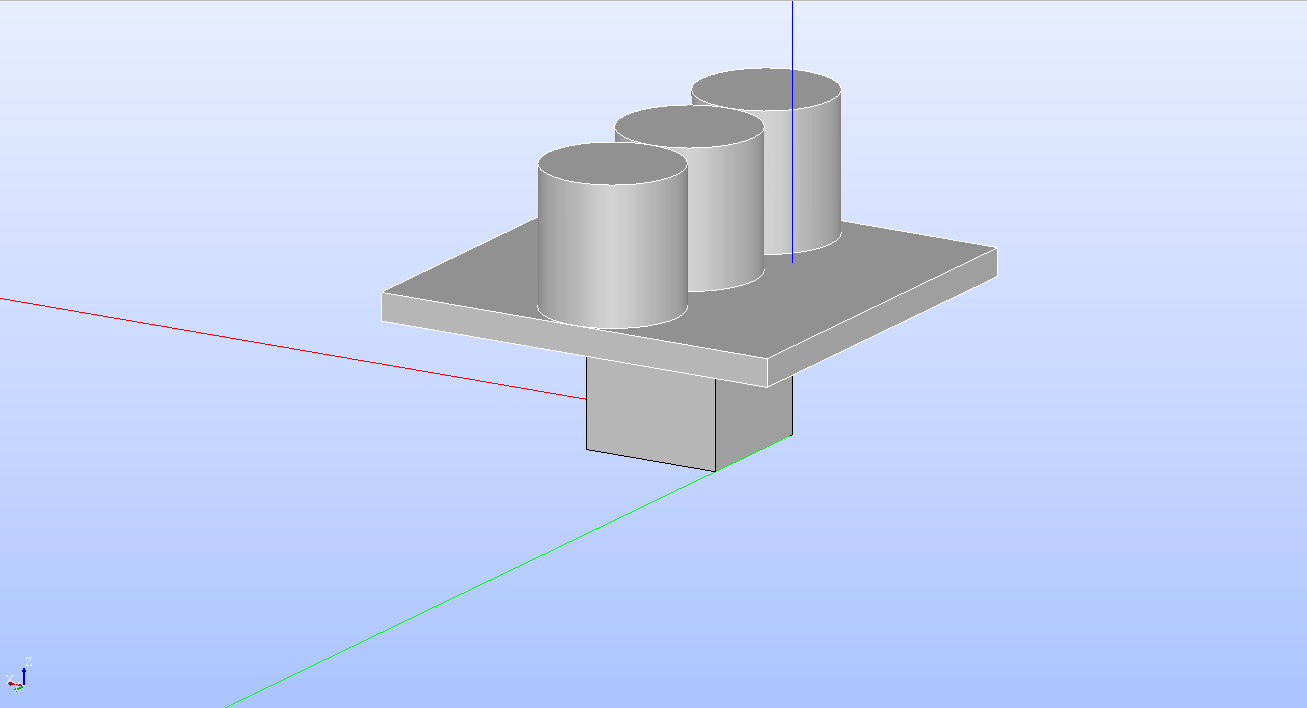
\includegraphics[width=0.5\linewidth]{1.3.png}
		\caption{Модель геометрии 3}
	\end{center}
\end{figure}
\newpage

\begin{figure}[h]
	\begin{center}
		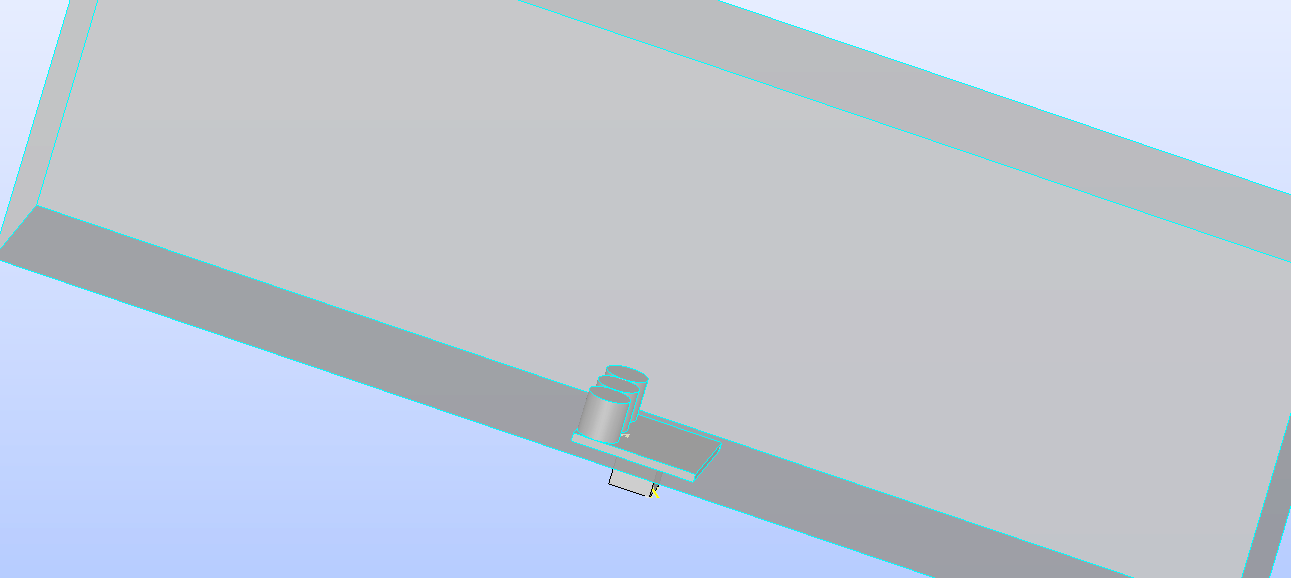
\includegraphics[width=0.5\linewidth]{2.1.png}
		\caption{Модель геометрии 1} %% подпись к рисунку
	\end{center}
\end{figure}
\begin{figure}[h]
	\begin{center}
		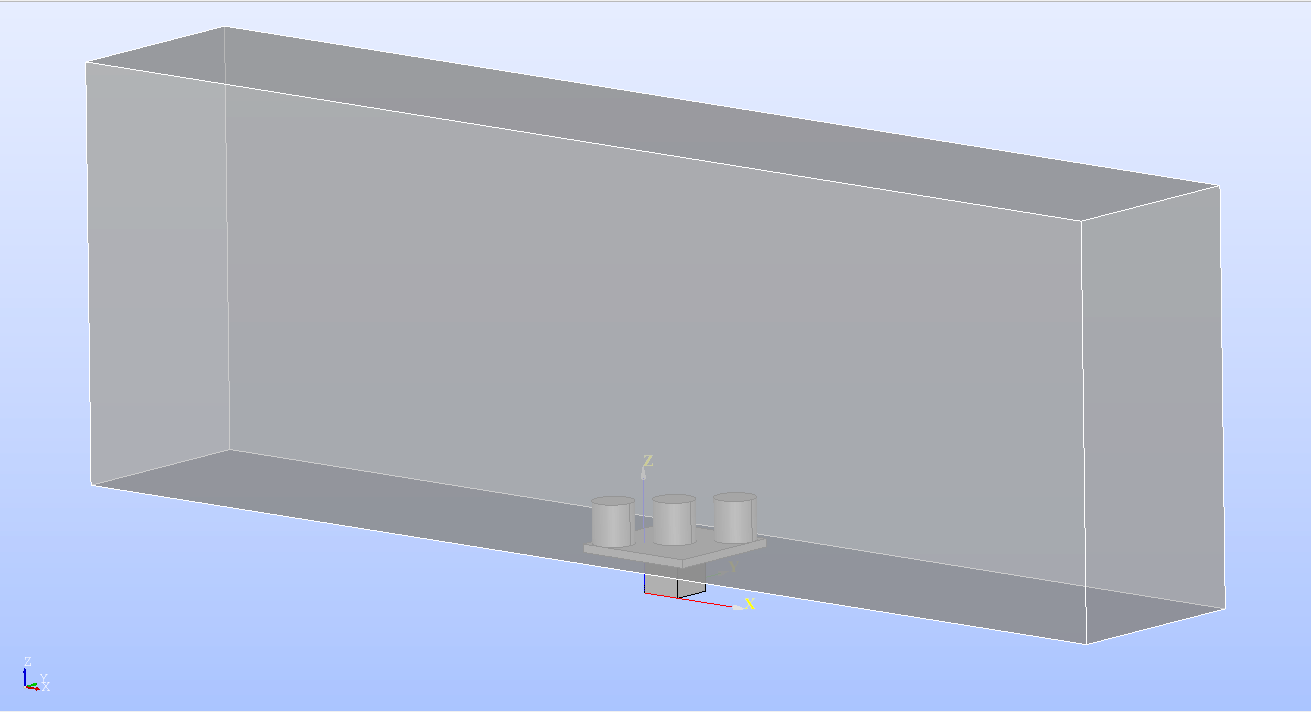
\includegraphics[width=0.5\linewidth]{2.2.png}
		\caption{Модель геометрии 2}
	\end{center}
\end{figure}
\newpage
\begin{figure}[h]
	\begin{center}
		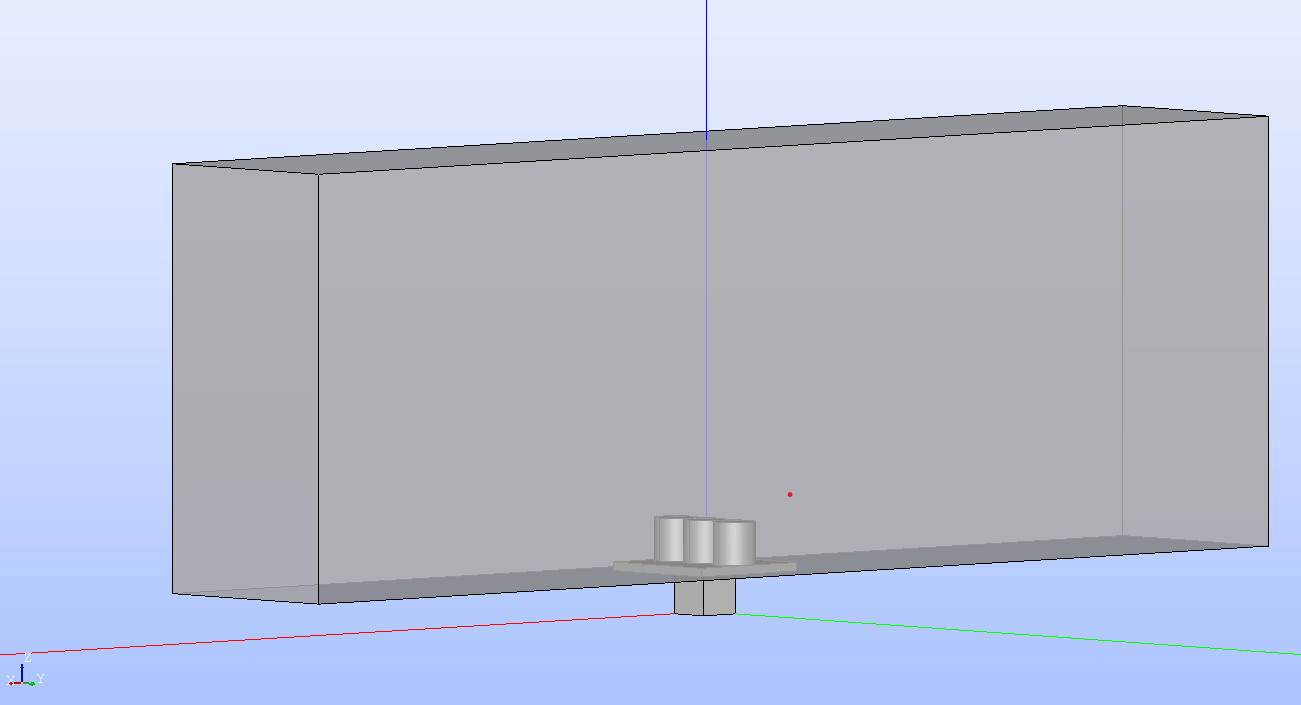
\includegraphics[width=0.5\linewidth]{2.3.png}
		\caption{Модель геометрии 3}
	\end{center}
\end{figure}

\par
В данных моделях части радиатора (3 цилиндрических элемента) являются подвижными и могут быть сдвинуты по оси Ox. Их радиус основания равен 5 мм, а высота 10 мм. 
Размеры подложки радиатора по ширине и длине 30 мм, а по высоте 2 мм. Нагреватель представляет собой куб с длиной ребра 10 мм и объемной плотностью источников тепла 2.94 * $10^7$ Вт/$м^3$. 
Скорость потока воздуха 5.6 м/с. Воздух находится в параллелепипеде размерами 300 мм по длине, 50 мм по ширине и 100 мм по высоте. Начальная температура –296.9 К. Параметры материалов приведены в таблице 1 \cite{aHeatTranserf}.

\begin{table}[h]
	\begin{tabular}{|l|l|l|l|}
		\hline
		                                          & Нагреватель & Радиатор & Воздух        \\
		Плотность {[}кг/$м^3${]}                  & 1280        & 2700     & 1.196         \\
		\hline
		Cp   {[}Дж/кг*К{]}                        & 1004        & 900      & 1005          \\
		\hline
		Коэффициент теплопроводности {[}Вт/м*К{]} & 80          & 200      &               \\
		\hline
		Молекулярная масса {[}г/моль{]}           & 50          & 27       & 28.9          \\
		\hline
		Вязкость {[}кг/м*с{]}                     &             &          & $1.8*10^{-5}$ \\
		\hline
		Число Прандтля                            &             &          & 0.7           \\
		\hline
	\end{tabular}
	\caption{Параметры задачи} %% подпись к рисунку
\end{table}

Затем по модели была построена сетка c уплотнением в области радиатора и нагревателя и произведено разбиение на регионы:

\begin{figure}[h]
	\begin{center}
		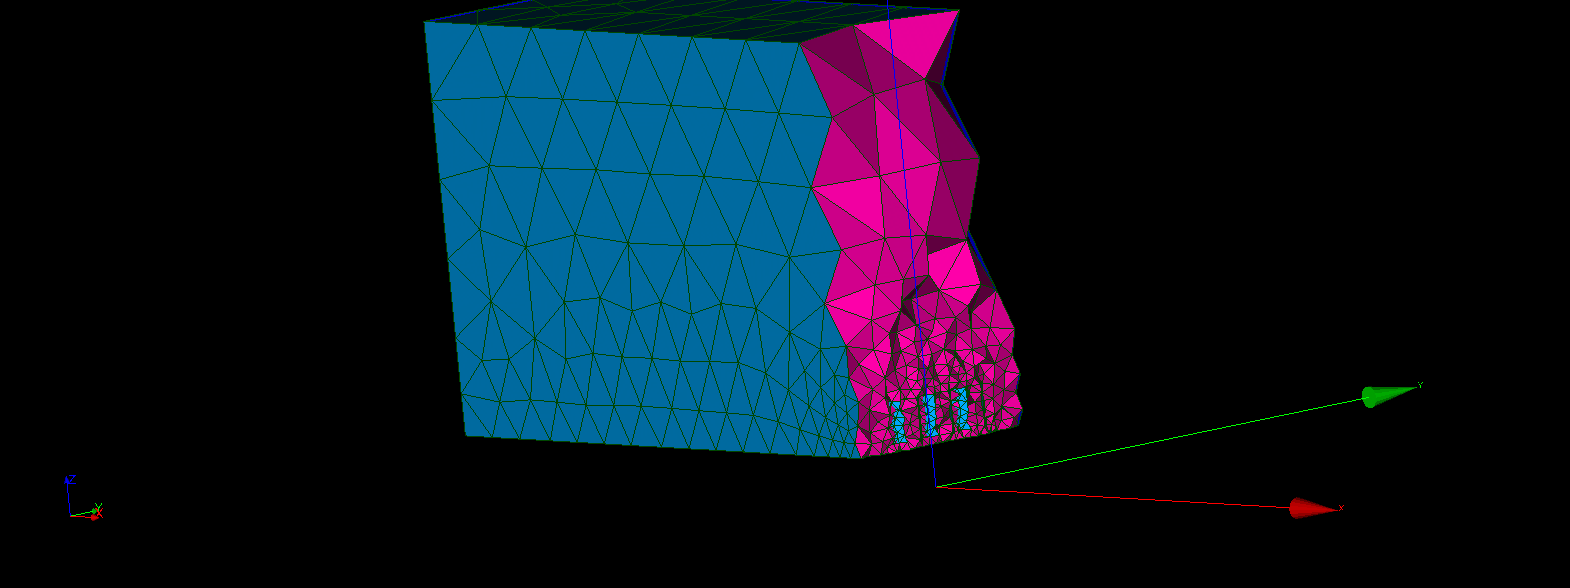
\includegraphics[width=0.35\linewidth]{3.png}
		\caption{Сетка модели 1} %% подпись к рисунку
	\end{center}
\end{figure}

\par
Для численного решения задачи используется решатель chtMultiRegionFoam.
Он применяется для расчета теплообмена между жидкостью/газом и твердым телом. А также для моделирования сложных задач, связанных с теплопередачей и теплообменом в многорегиональных системах \cite{wChtMultiRegionFoam}.
Для каждого региона задавались начальные и граничные условия. Были также заданы дополнительные функции для анализа \cite{aHeatTranserf}.
Для моделей были получены следующие результаты распределений по температурам:

\begin{figure}[h]
	\begin{center}
		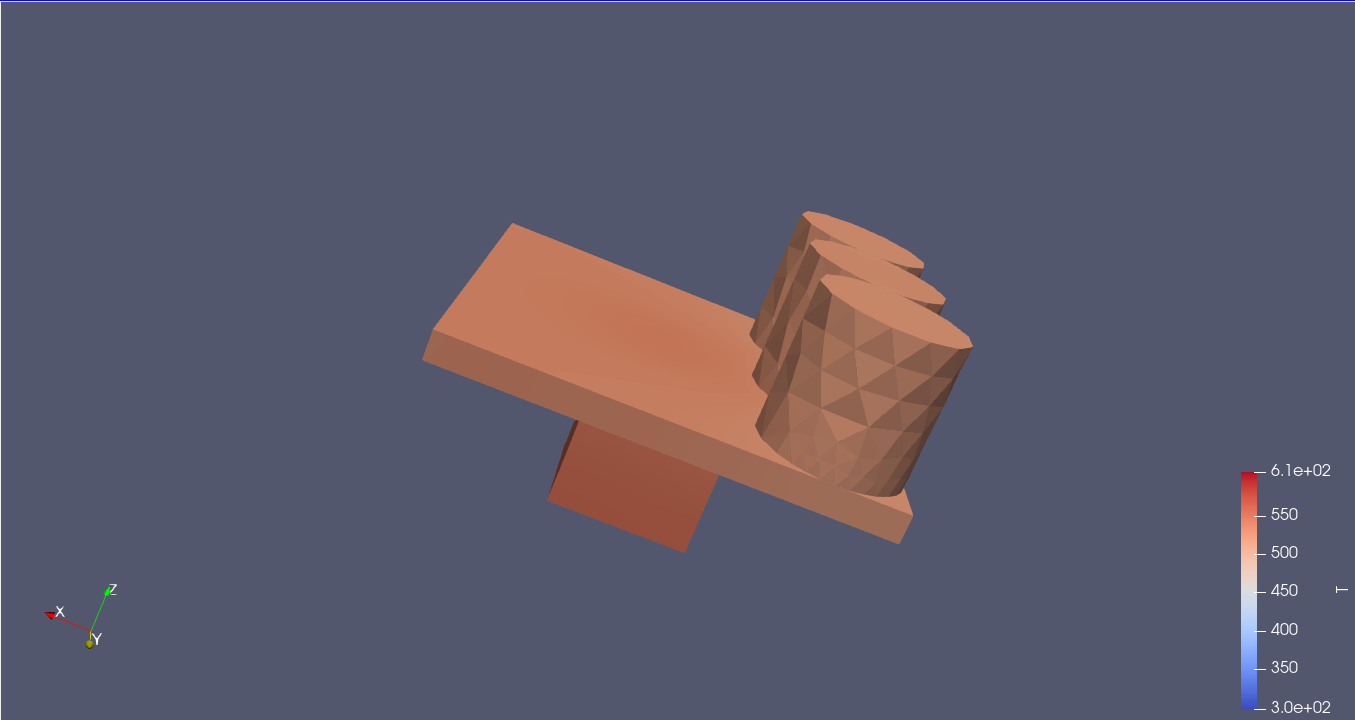
\includegraphics[width=0.45\linewidth]{5.1.png}
		\caption{Распределение температуры для модели 1} %% подпись к рисунку
	\end{center}
\end{figure}

\begin{figure}[h]
	\begin{center}
		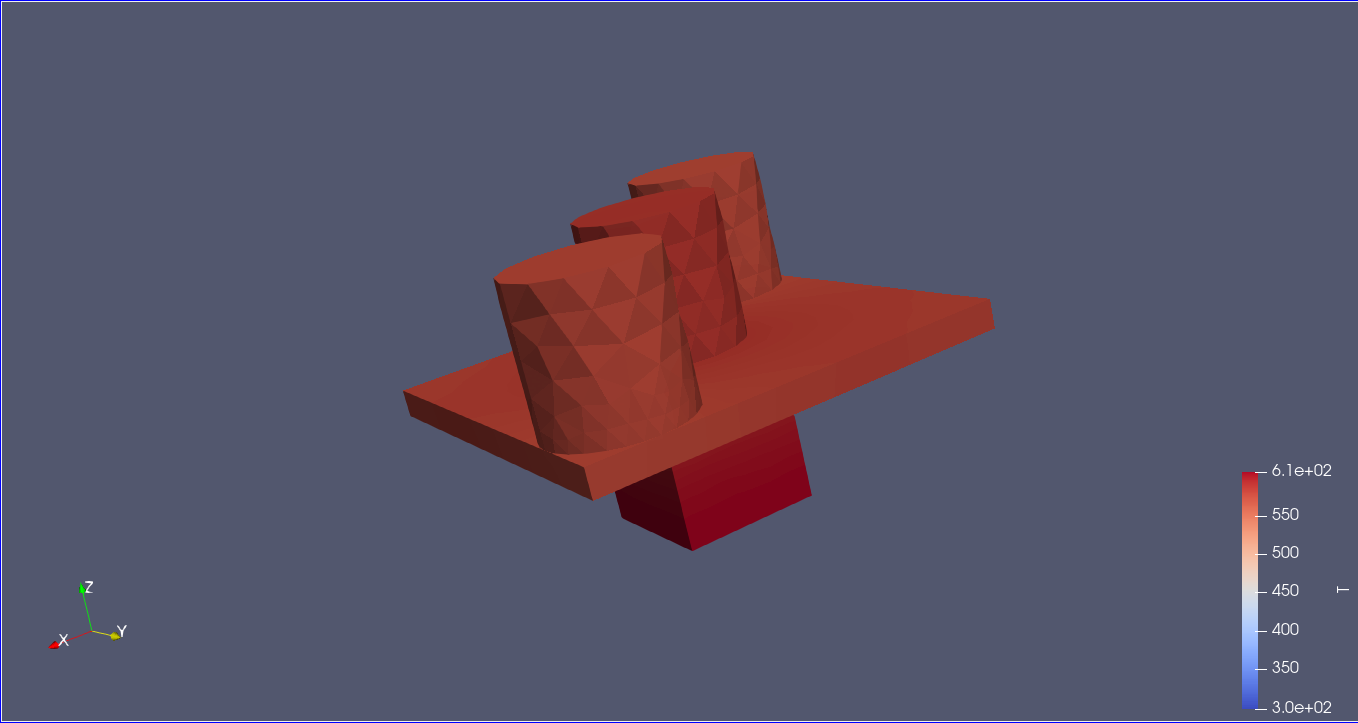
\includegraphics[width=0.45\linewidth]{5.2.png}
		\caption{Распределение температуры для модели 2} %% подпись к рисунку
	\end{center}
\end{figure}

\begin{figure}[h]
	\begin{center}
		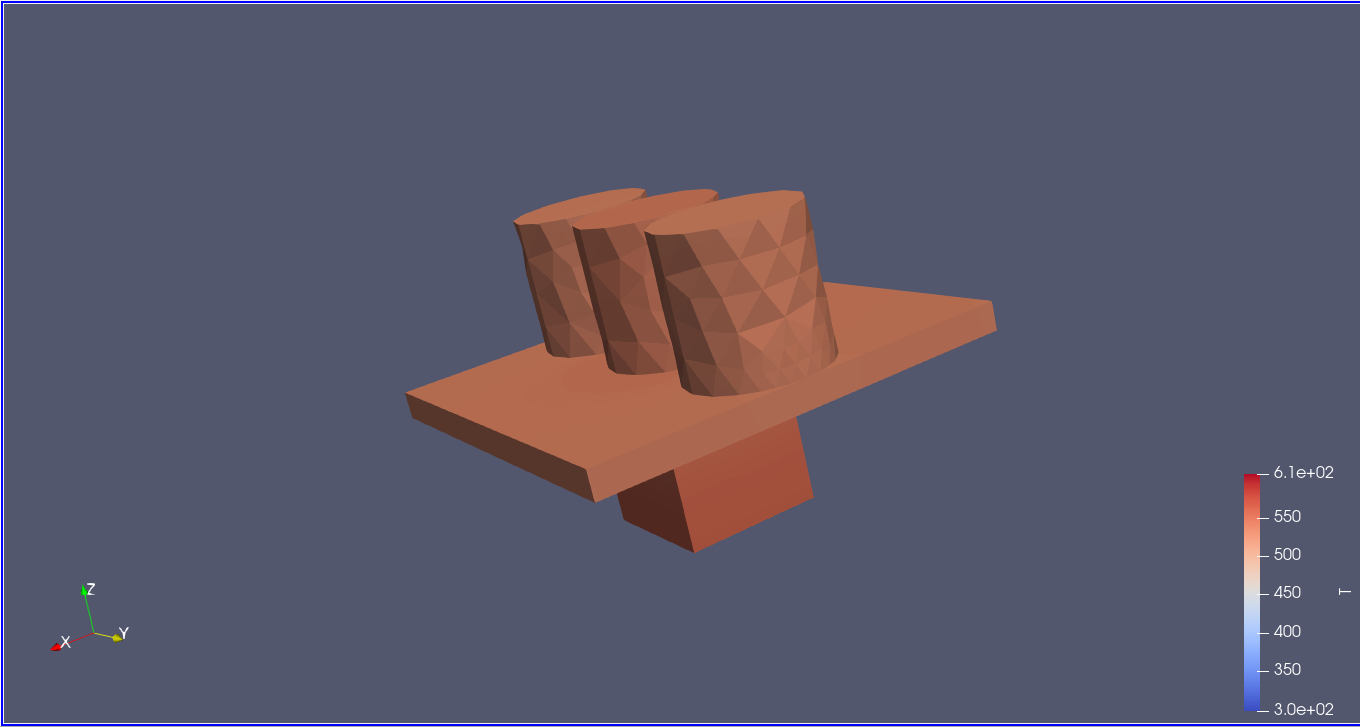
\includegraphics[width=0.45\linewidth]{5.3.png}
		\caption{Распределение температуры для модели 3} %% подпись к рисунку
	\end{center}
\end{figure}

\newpage
Были получены следующие результаты для моделей:
\begin{enumerate}
	\item \textbf{Первая модель:}
	      \begin{itemize}
		      \item Средняя температура радиатора: 508.381 К
		      \item Средняя температура нагревателя: 533.363 К
		      \item Средняя температура интерфейса между нагревателем и радиатором: 521.537 К
	      \end{itemize}
	\item \textbf{Вторая модель:}
	      \begin{itemize}
		      \item Средняя температура радиатора: 555.23 К
		      \item Средняя температура нагревателя: 576.306 К
		      \item Средняя температура интерфейса между нагревателем и радиатором: 564.451 К
	      \end{itemize}
	\item \textbf{Третья модель:}
	      \begin{itemize}
		      \item Средняя температура радиатора: 519.325 К
		      \item Средняя температура нагревателя: 537.741 К
		      \item Средняя температура интерфейса между нагревателем и радиатором: 525.862 К
	      \end{itemize}
\end{enumerate}

Построены графики температуры в нагревателе:
\newpage
\begin{figure}[h]
	\begin{center}
		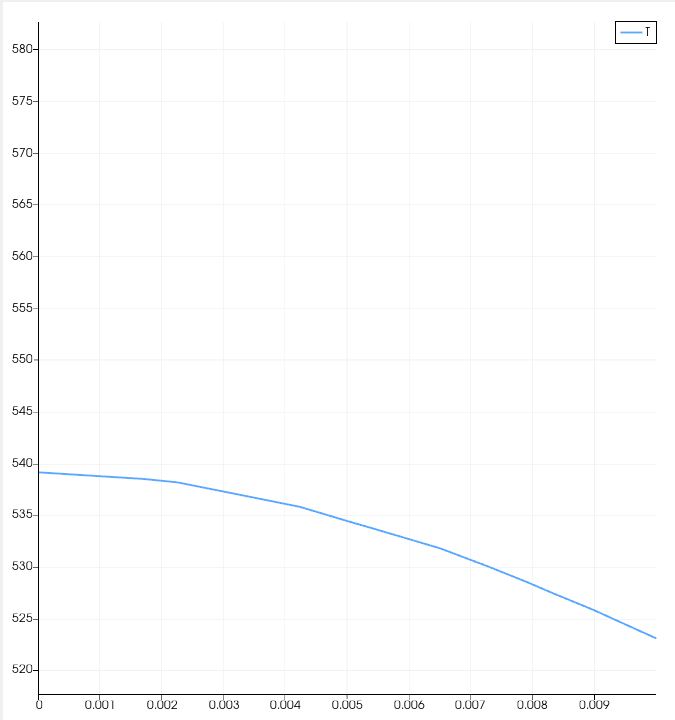
\includegraphics[width=0.4\linewidth]{6.1.png}
		\caption{Распределение температуры в нагревателе для модели 1} %% подпись к рисунку
	\end{center}
\end{figure}
\begin{figure}[h]
	\begin{center}
		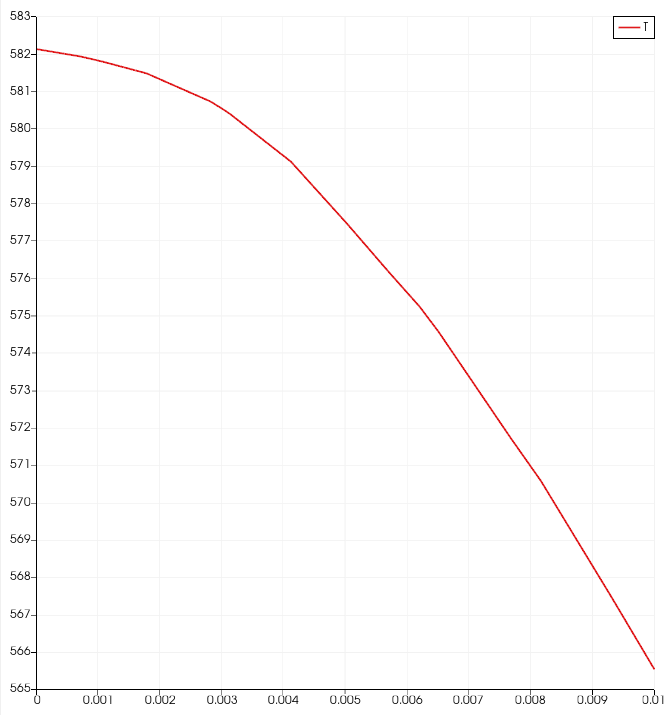
\includegraphics[width=0.4\linewidth]{6.2.png}
		\caption{Распределение температуры в нагревателе для модели 2} %% подпись к рисунку
	\end{center}
\end{figure}
\newpage
\begin{figure}[h]
	\begin{center}
		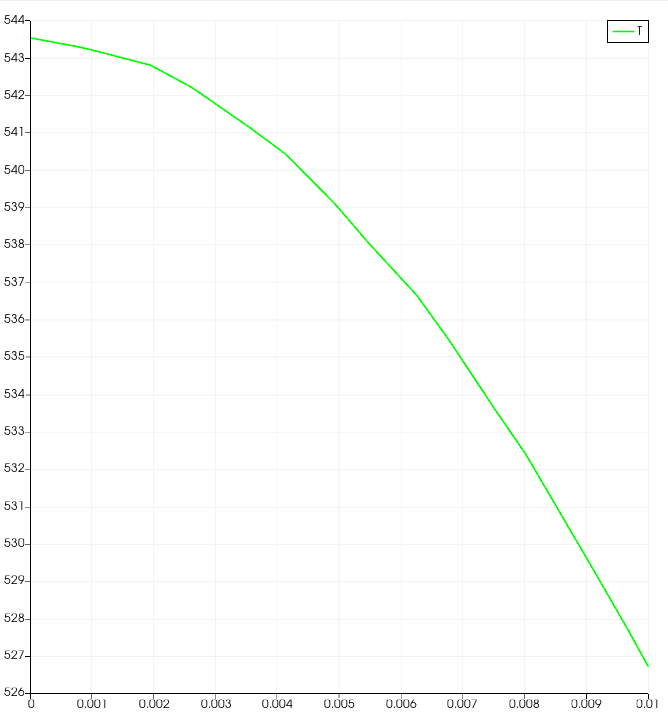
\includegraphics[width=0.4\linewidth]{6.3.png}
		\caption{Распределение температуры в нагревателе для модели 3} %% подпись к рисунку
	\end{center}
\end{figure}
\begin{figure}[h]
	\begin{center}
		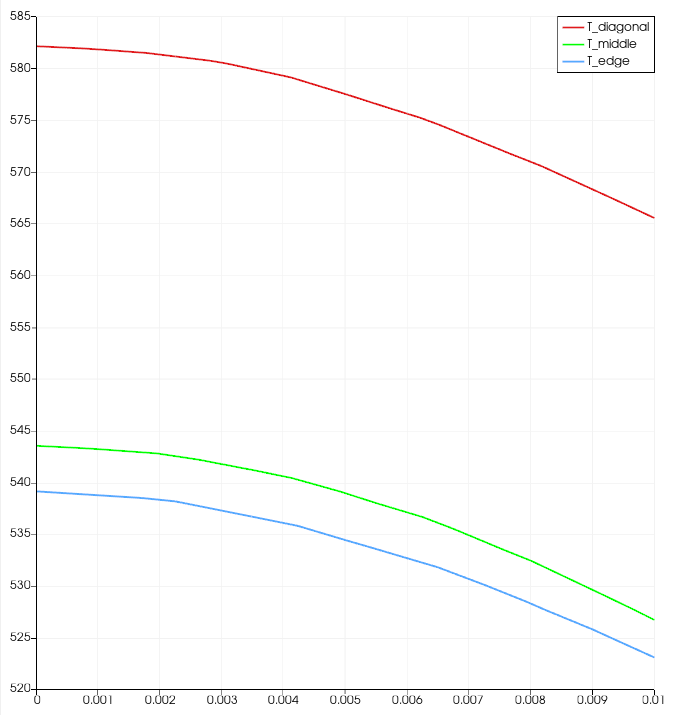
\includegraphics[width=0.4\linewidth]{6.png}
		\caption{Распределение температур в нагревателях для всех моделей} %% подпись к рисунку
	\end{center}
\end{figure}

\newpage
\par
Затем было проведено 2000 итераций расчета. Для отслеживания сходимости во время проведения расчета были построены следующие графики (пример для модели 1):
\begin{figure}[h]
	\begin{center}
		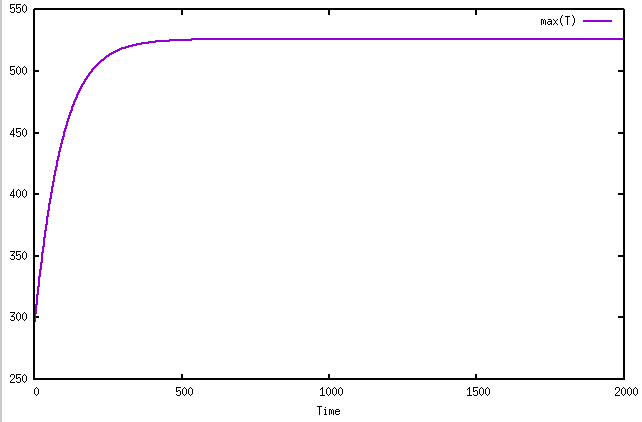
\includegraphics[width=0.35\linewidth]{11.1.png}
		\caption{Зависимость максимальной температуры радиатора от шага} %% подпись к рисунку
	\end{center}
\end{figure}
\begin{figure}[h]
	\begin{center}
		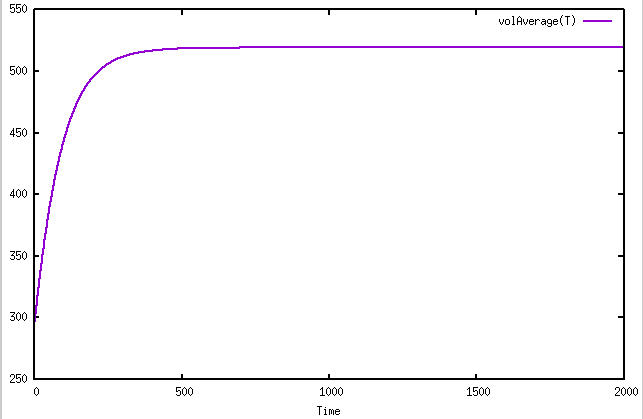
\includegraphics[width=0.35\linewidth]{12.1.png}
		\caption{Зависимость средней температуры радиатора от шага} %% подпись к рисунку
	\end{center}
\end{figure}
\begin{figure}[h]
	\begin{center}
		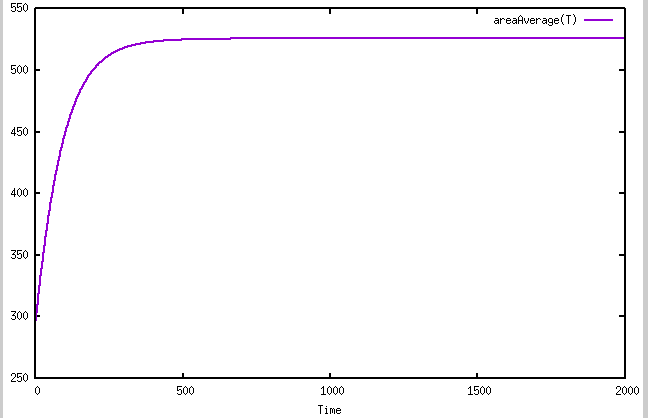
\includegraphics[width=0.35\linewidth]{13.1.png}
		\caption{Зависимость средней температуры интерфейса между нагревателем и радиатором от шага} %% подпись к рисунку
	\end{center}
\end{figure}
\newpage
\begin{figure}[h]
	\begin{center}
		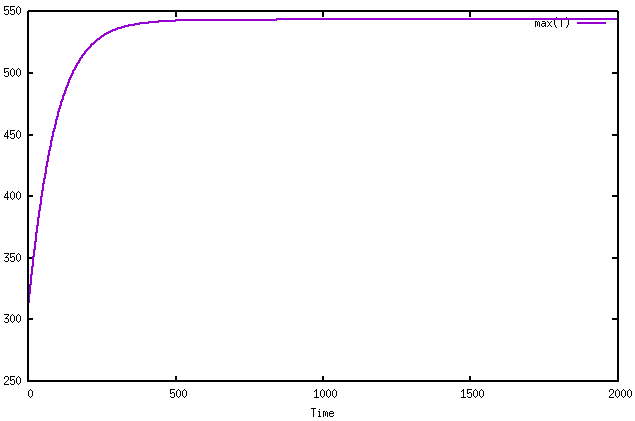
\includegraphics[width=0.4\linewidth]{14.1.png}
		\caption{Зависимость максимальной температуры нагревателя от шага} %% подпись к рисунку
	\end{center}
\end{figure}
\begin{figure}[h]
	\begin{center}
		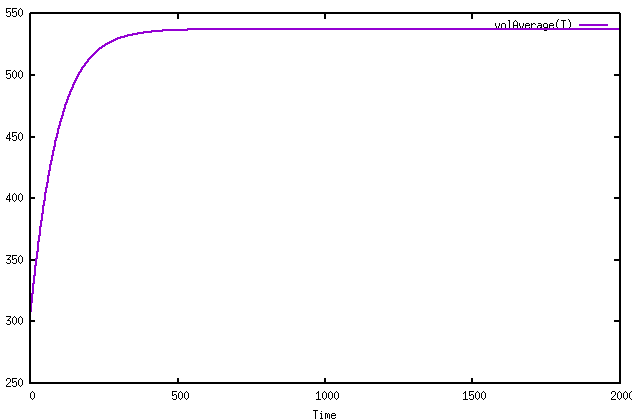
\includegraphics[width=0.4\linewidth]{15.1.png}
		\caption{Зависимость средней температуры нагревателя от шага} %% подпись к рисунку
	\end{center}
\end{figure}

\par
Далее были построены графики распределений температуры в центральном сечении:

\begin{figure}[h]
	\begin{center}
		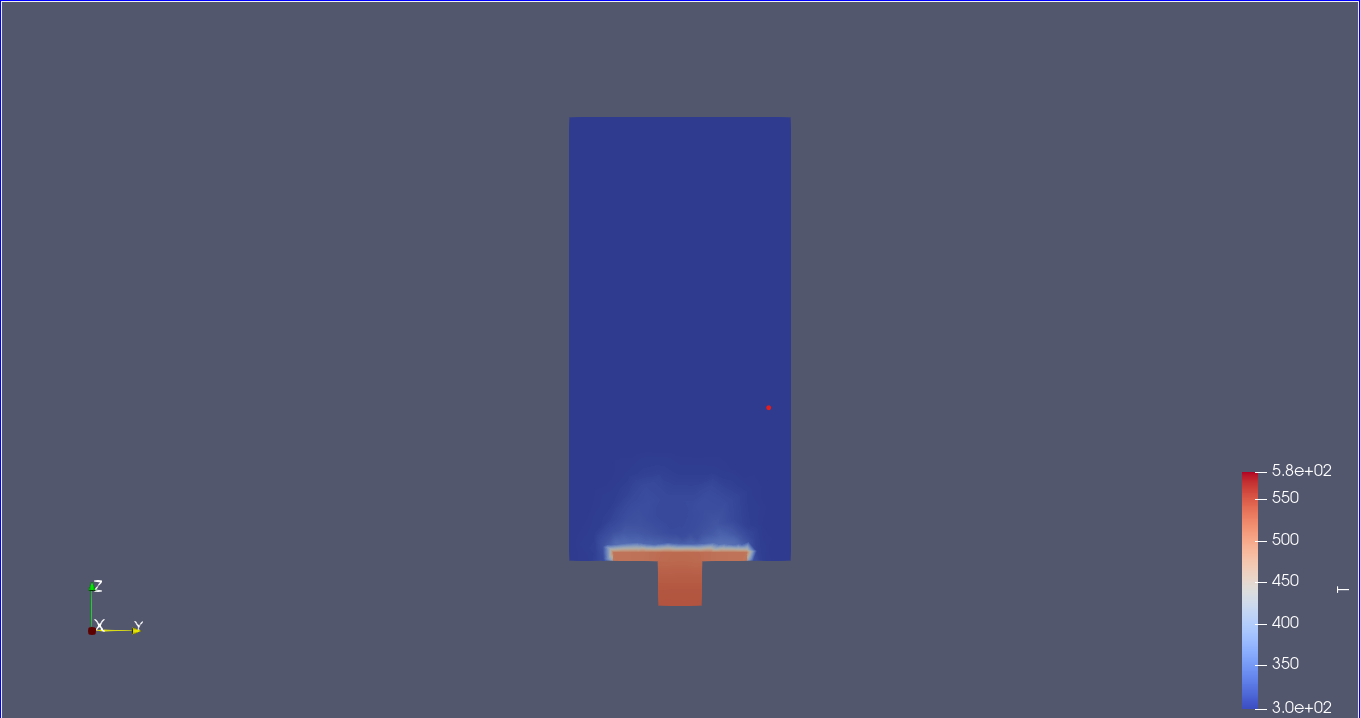
\includegraphics[width=0.4\linewidth]{7.1.png}
		\caption{Распределение температуры для модели 1} %% подпись к рисунку
	\end{center}
\end{figure}

\begin{figure}[h]
	\begin{center}
		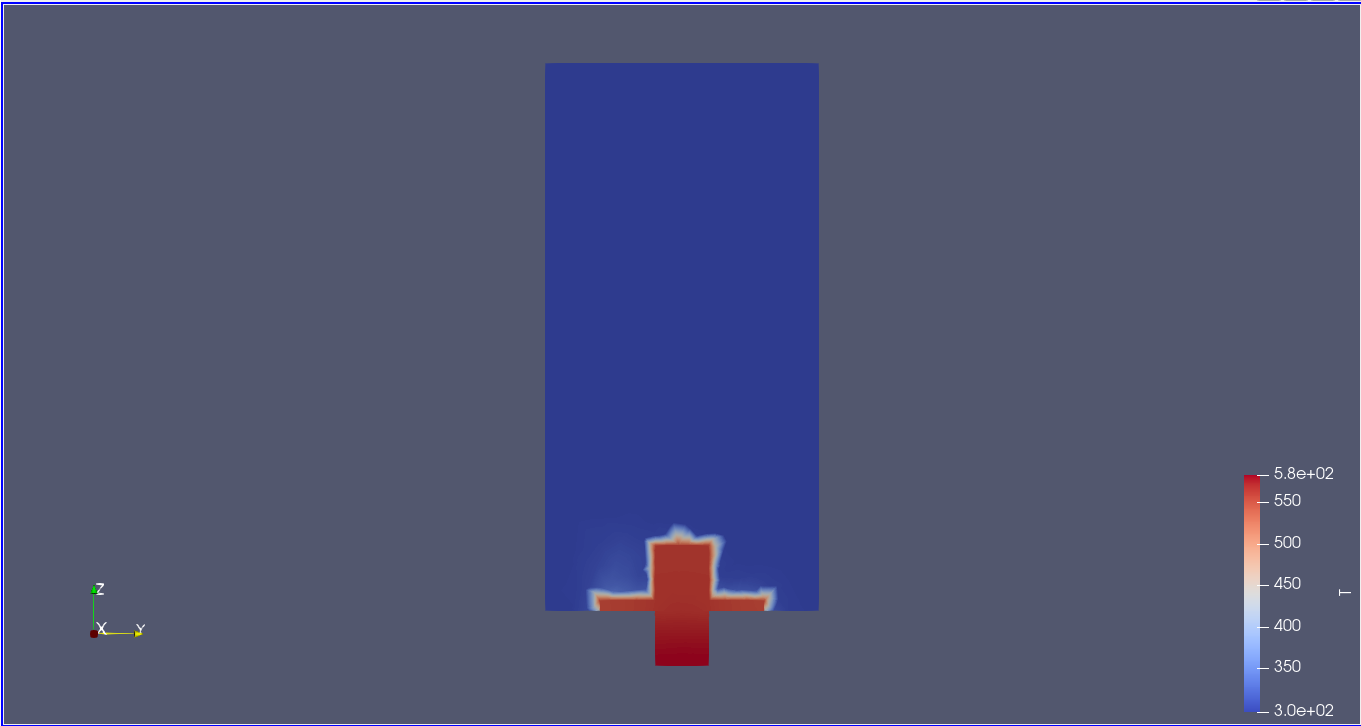
\includegraphics[width=0.4\linewidth]{7.2.png}
		\caption{Распределение температуры для модели 2} %% подпись к рисунку
	\end{center}
\end{figure}
\newpage
\begin{figure}[h]
	\begin{center}
		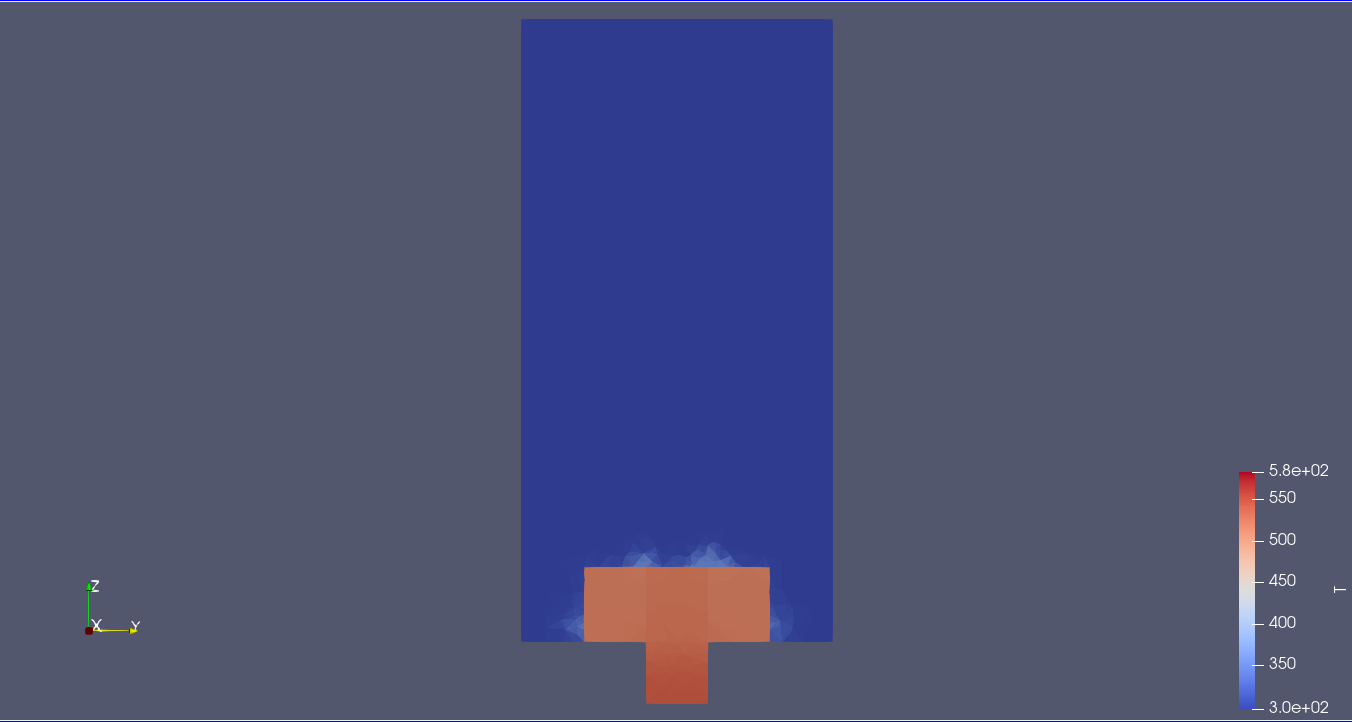
\includegraphics[width=0.4\linewidth]{7.3.png}
		\caption{Распределение температуры для модели 3} %% подпись к рисунку
	\end{center}
\end{figure}

\par
И графики распределений скоростей:
\begin{figure}[h]
	\begin{center}
		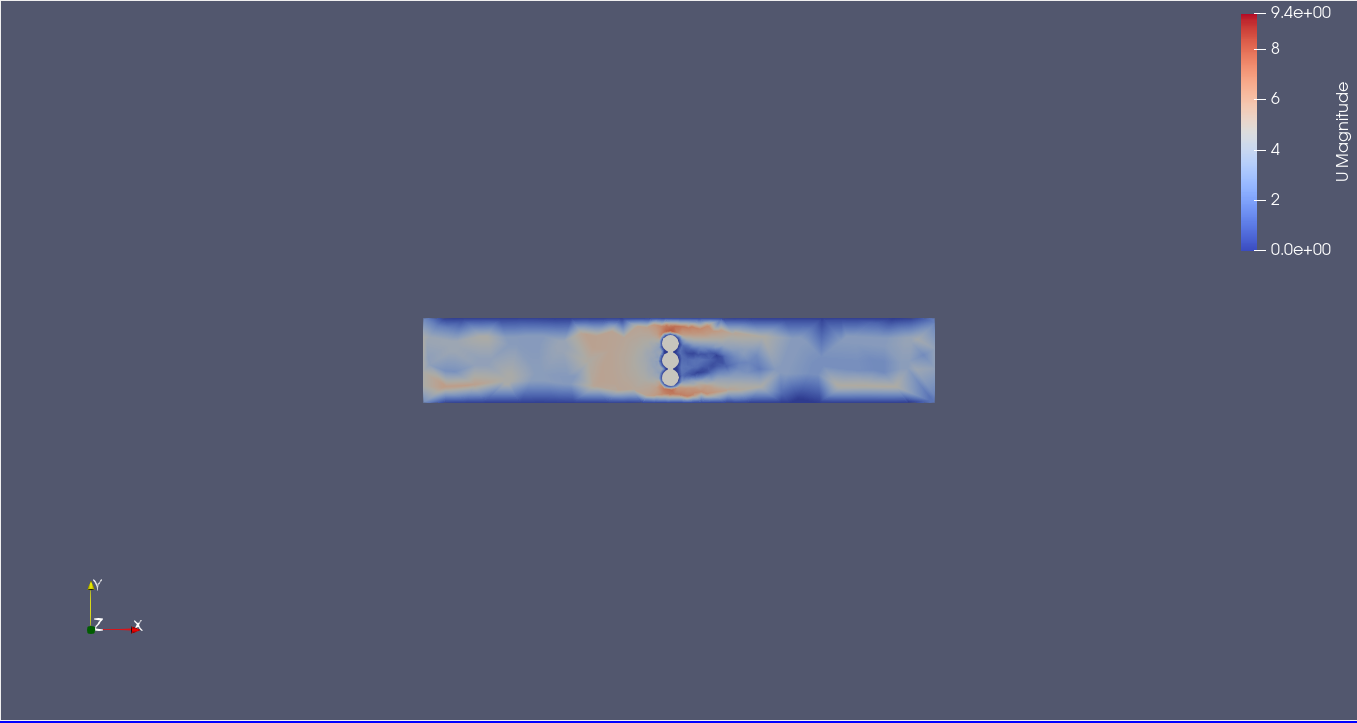
\includegraphics[width=0.4\linewidth]{8.1.png}
		\caption{Распределение скоростей для модели 1} %% подпись к рисунку
	\end{center}
\end{figure}

\begin{figure}[h]
	\begin{center}
		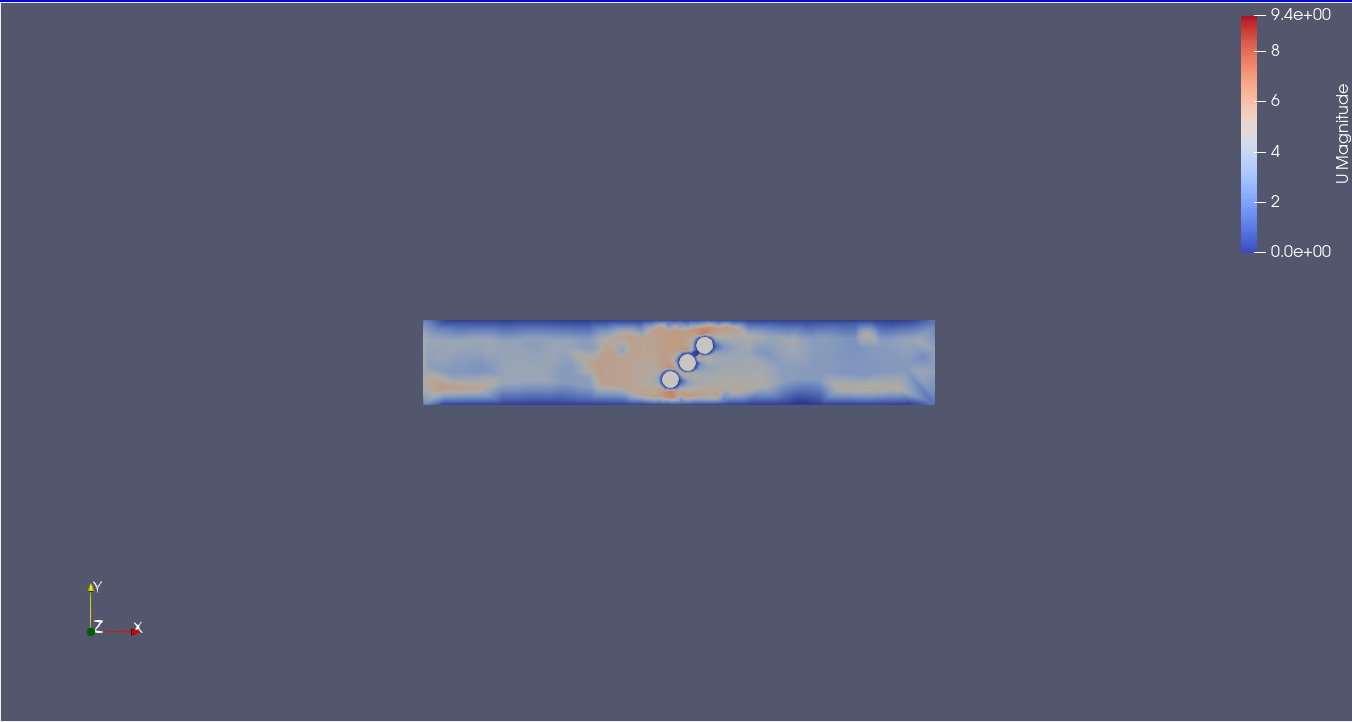
\includegraphics[width=0.4\linewidth]{8.2.png}
		\caption{Распределение скоростей для модели 2} %% подпись к рисунку
	\end{center}
\end{figure}
\newpage
\begin{figure}[h]
	\begin{center}
		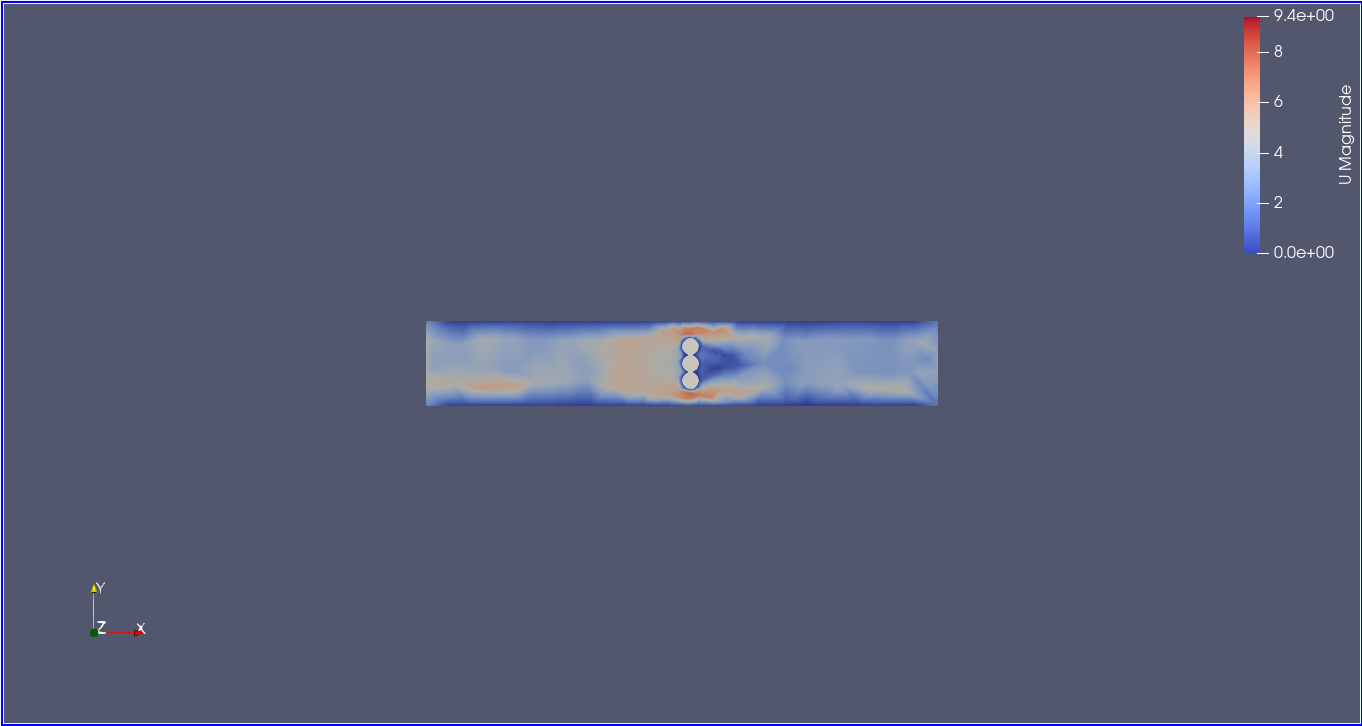
\includegraphics[width=0.4\linewidth]{8.3.png}
		\caption{Распределение скоростей для модели 3} %% подпись к рисунку
	\end{center}
\end{figure}
\begin{figure}[h]
	\begin{center}
		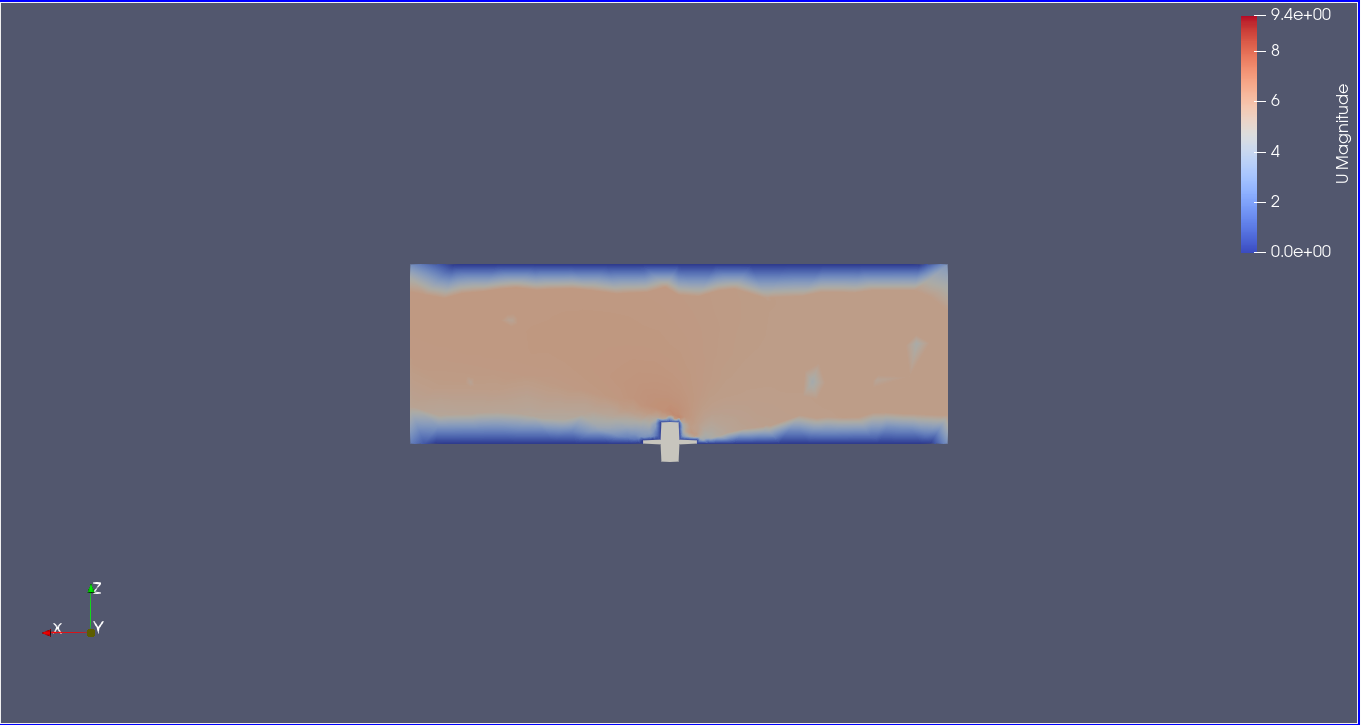
\includegraphics[width=0.4\linewidth]{9.png}
		\caption{Распределение скоростей для модели 1} %% подпись к рисунку
	\end{center}
\end{figure}

\section{Проблема с автоматической генерацией сетки в SALOME}

В ходе исследованиЯ при перегенерации геометрии в SALOME, используя дамп скрипта, мы получали сетку с ошибками из-за нарушения идентификаторов (ID) сущностей.

Для решения данной проблемы был использован Python API в SALOME и применялись следующие методы:
\subsection{\texttt{SubShapeAllIDs}}

Функция \texttt{SubShapeAllIDs} в Python API SALOME используется для получения всех идентификаторов (ID) подформ в геометрии. Это полезно, когда необходимо провести операции с каждой подформой в модели.

Пример использования:
\begin{verbatim}
subshape_ids = geompy.SubShapeAllIDs(main_shape)
print(f"ID подформ: {subshape_ids}")
\end{verbatim}

В данном примере \texttt{main\_shape} - это главная форма в вашей геометрии.

\subsection{\texttt{GetShapesOnBoxIDs}}

Функция \texttt{GetShapesOnBoxIDs} возвращает идентификаторы форм, которые содержатся внутри заданного объема, определенного прямоугольным параллелепипедом.

Пример использования:
\begin{verbatim}
box = geompy.MakeBox(0, 0, 0, 10, 10, 10)
shapes_inside_box_ids = geompy.GetShapesOnBoxIDs(main_shape, box)
print(f"ID форм внутри прямоугольного параллелепипеда: {shapes_inside_box_ids}")
\end{verbatim}

Здесь \texttt{main\_shape} - это опять же главная форма, а \texttt{box} - созданный прямоугольный параллелепипед.

\subsection{\texttt{GetShapesOnPlaneWithLocationIDs}}

Функция \texttt{GetShapesOnPlaneWithLocationIDs} возвращает идентификаторы форм, которые пересекают заданную плоскость.

Пример использования:
\begin{verbatim}
plane = geompy.MakePlane(0, 0, 1, 0)
shapes_on_plane_ids = geompy.GetShapesOnPlaneWithLocationIDs(main_shape, plane)
print(f"ID форм, пересекаемых плоскостью: {shapes_on_plane_ids}")
\end{verbatim}

В этом примере \texttt{main\_shape} - главная форма, а \texttt{plane} - созданная плоскость.

Используя эти методы, мы смогли стабилизировать процесс генерации сетки, обеспечивая постоянство идентификаторов форм даже при обновлении геометрии. Это решение позволило нам успешно использовать скрипт в дальнейших этапах нашего исследования.

\section{Автоматизированный процесс генерации сетки и расчета}

На данном этапе работы рассматривается процесс автоматизации генерации сетки в программе SALOME и выполнения расчетов в OpenFOAM для различных комбинаций параметров. Ключевыми параметрами, подлежащими варьированию, являются \\ \texttt{shift\_first\_cylinder} и \texttt{shift\_second\_cylinder}.

Переменная \texttt{shift\_first\_cylinder} представляет собой сдвиг первого цилиндра в радиаторе, а \texttt{shift\_second\_cylinder} — сдвиг второго цилиндра. Эти параметры влияют на геометрию радиатора и, следовательно, на условия теплообмена в системе.

Скрипт создает уникальное имя для каждой комбинации параметров и затем копирует исходный кейс в новую директорию. После этого SALOME запускается в режиме командной строки для выполнения генерации сетки с учетом новой геометрии, заданной параметрами сдвига цилиндров. Далее запускаются соответствующие bash-скрипты для выполнения кейса в OpenFOAM.

После завершения расчета, автоматически извлекаются результаты. Сценарий ищет и анализирует файл с данными теплообмена в постпроцессинговой директории. Это позволяет собирать и систематизировать конечные результаты для каждой конфигурации геометрии. Такой подход обеспечивает эффективный анализ влияния различных параметров на теплоотдачу системы.

\section{Особенности фиксации и движения цилиндров}

Необходимо отметить, что в проведенных исследованиях у нас было три цилиндра в системе. Тем не менее, третий цилиндр был зафиксирован в положении (0, 0), и двигались только два оставшихся цилиндра. Такой выбор сделан с целью упростить визуализацию и анализ результатов.

Такой подход облегчает анализ и интерпретацию результатов, обеспечивая более ясное представление о влиянии конкретных параметров на эффективность теплообмена в рассматриваемой системе.

\section{Первые результаты}

На основе автоматизированного процесса были получены первые результаты, охватывающие 25 точек варьирования параметров. Исследуемые параметры \texttt{shift\_first\_cylinder} и \texttt{shift\_second\_cylinder} изменялись от 0 до 20 с шагом 5. Эти значения представляют различные комбинации сдвигов цилиндров в радиаторе, что отражает влияние геометрических параметров на теплоотдачу системы.

\begin{figure}[h]
	\begin{center}
		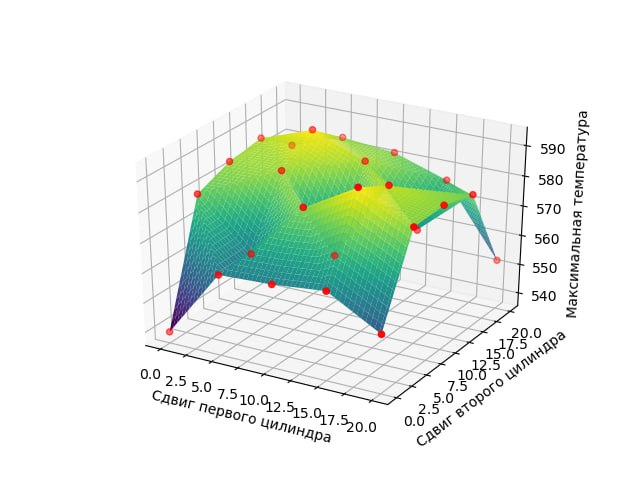
\includegraphics[width=0.4\linewidth]{16.1.jpg}
		\caption{Зависимость максимальной температуры нагревателя от сдвигов цилиндров} %% подпись к рисунку
	\end{center}
\end{figure}

\begin{figure}[h]
	\begin{center}
		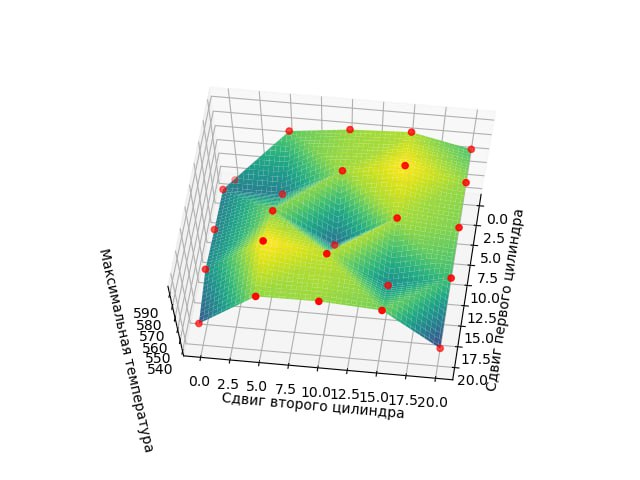
\includegraphics[width=0.4\linewidth]{16.2.jpg}
		\caption{Зависимость максимальной температуры нагревателя от сдвигов цилиндров} %% подпись к рисунку
	\end{center}
\end{figure}
\newpage
\begin{figure}[h]
	\begin{center}
		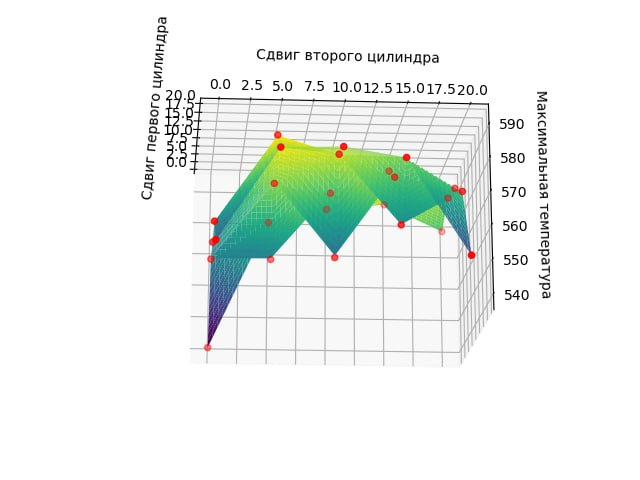
\includegraphics[width=0.4\linewidth]{16.3.jpg}
		\caption{Зависимость максимальной температуры нагревателя от сдвигов цилиндров} %% подпись к рисунку
	\end{center}
\end{figure}

Для улучшения визуализации и наглядности полученных данных была проведена интерполяция поверхности. Интерполированная поверхность дает представление о поведении системы в пространстве параметров и позволяет выявить области оптимальных значений для исследуемых параметров.

Этот этап анализа предоставляет первичное представление о влиянии сдвига цилиндров на теплообмен в системе.

\section{Оптимизация процесса расчета}

С целью оптимизации процесса расчета для большего количества точек был реализован многопоточный код на языке программирования Python. Для этого был использован модуль multiprocessing, который позволяет создавать и управлять параллельными процессами.

Прежде всего, были внесены некоторые изменения в существующий код. Введены параметры \texttt{shift\_third\_cylinder} и \texttt{all\_data} для адаптации к третьему цилиндру и сбору результатов в разделяемом словаре. Это позволило более гибко настраивать геометрию и эффективно собирать результаты расчетов.

С использованием модуля multiprocessing была реализована функция \texttt{run\_simulation}, которая выполняет расчет для каждой комбинации параметров в отдельном процессе. Результаты каждого процесса сохраняются в разделяемом словаре \texttt{all\_data}, где ключами являются уникальные идентификаторы (например, \texttt{\_0\_0\_0}), а значениями — результаты расчетов.

Затем, с использованием библиотеки Pool и метода \texttt{starmap}, были запущены отдельные процессы для каждой комбинации параметров. Это позволило распараллелить выполнение расчетов и значительно ускорить процесс.

Результаты расчетов были собраны в разделяемом словаре \texttt{all\_data}, который после завершения всех процессов может быть использован для анализа и построения интерполяции. Это позволяет обработать большой объем данных более эффективно, особенно при увеличении числа комбинаций параметров для анализа.

\section{Увеличение количества точек для анализа}

Оптимизация процесса расчета с использованием многопоточности значительно повысила эффективность анализа.

Так, на следующем этапе было проведено исследование с шагом 2, что дало 121 точку для анализа. Это уже более подробное и детальное исследование, что позволяет получить более точные представления о влиянии параметров на характеристики системы.

\begin{figure}[h]
	\begin{center}
		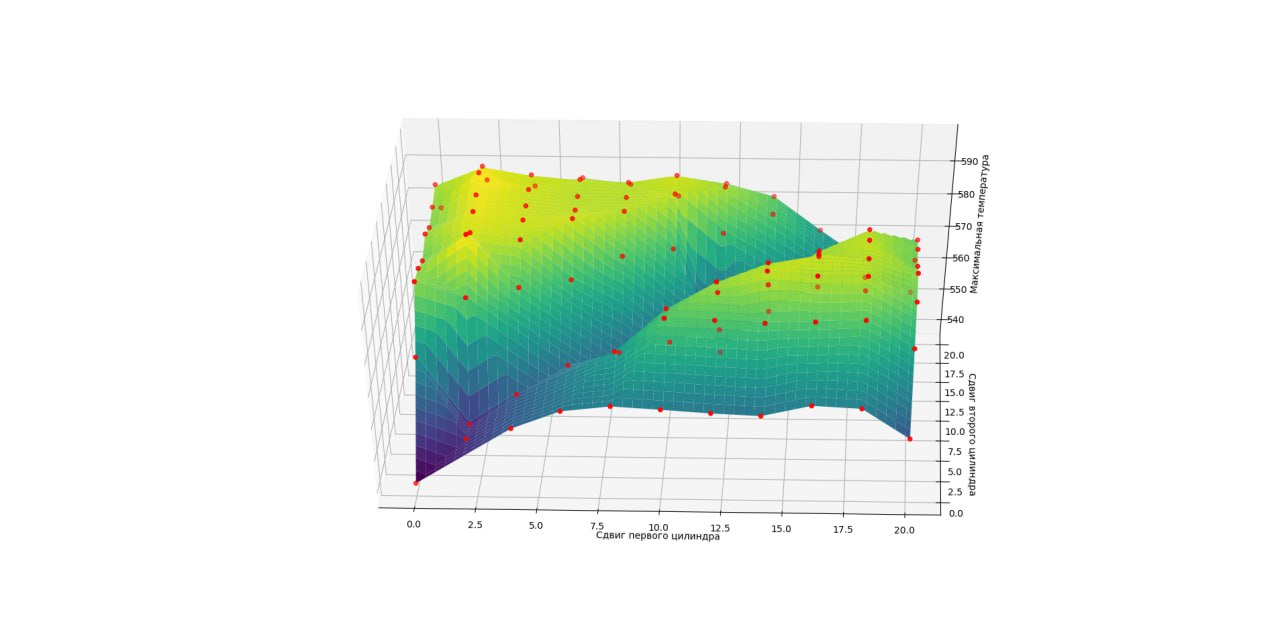
\includegraphics[width=0.4\linewidth]{17.1.jpg}
		\caption{Зависимость максимальной температуры нагревателя от сдвигов цилиндров (121 точка)} %% подпись к рисунку
	\end{center}
\end{figure}
\begin{figure}[h]
	\begin{center}
		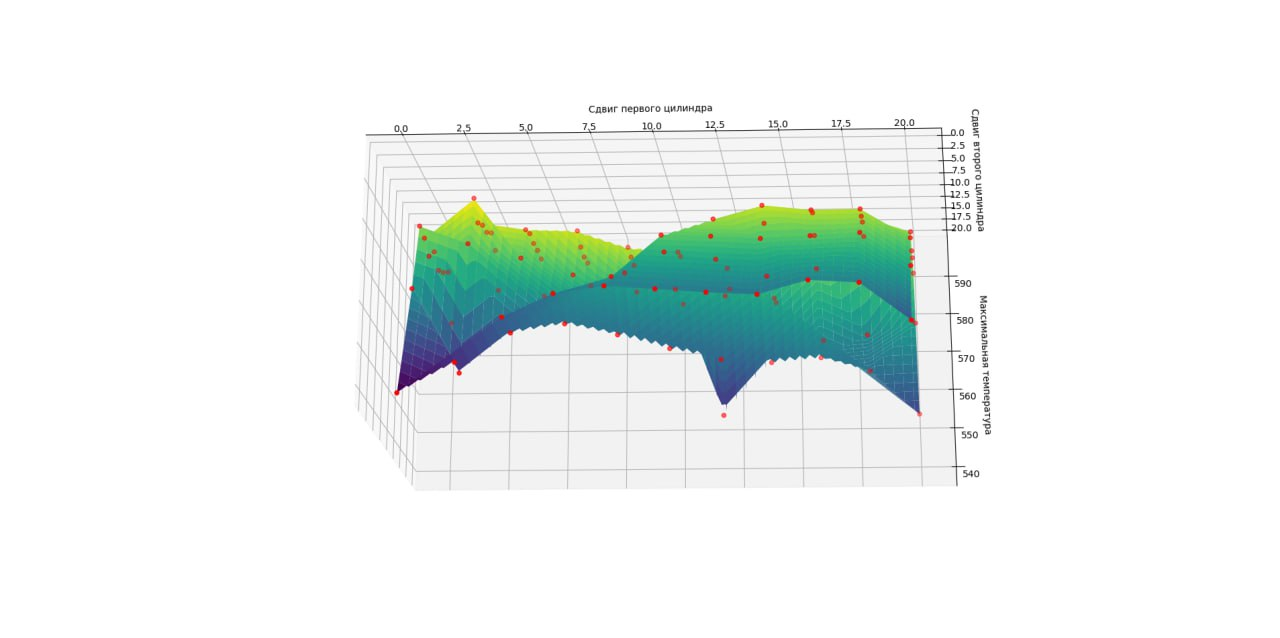
\includegraphics[width=0.4\linewidth]{17.2.jpg}
		\caption{Зависимость максимальной температуры нагревателя от сдвигов цилиндров (121 точка)} %% подпись к рисунку
	\end{center}
\end{figure}

Затем мы перешли к шагу 1, что привело к анализу 441 точки.

\begin{figure}[h]
	\begin{center}
		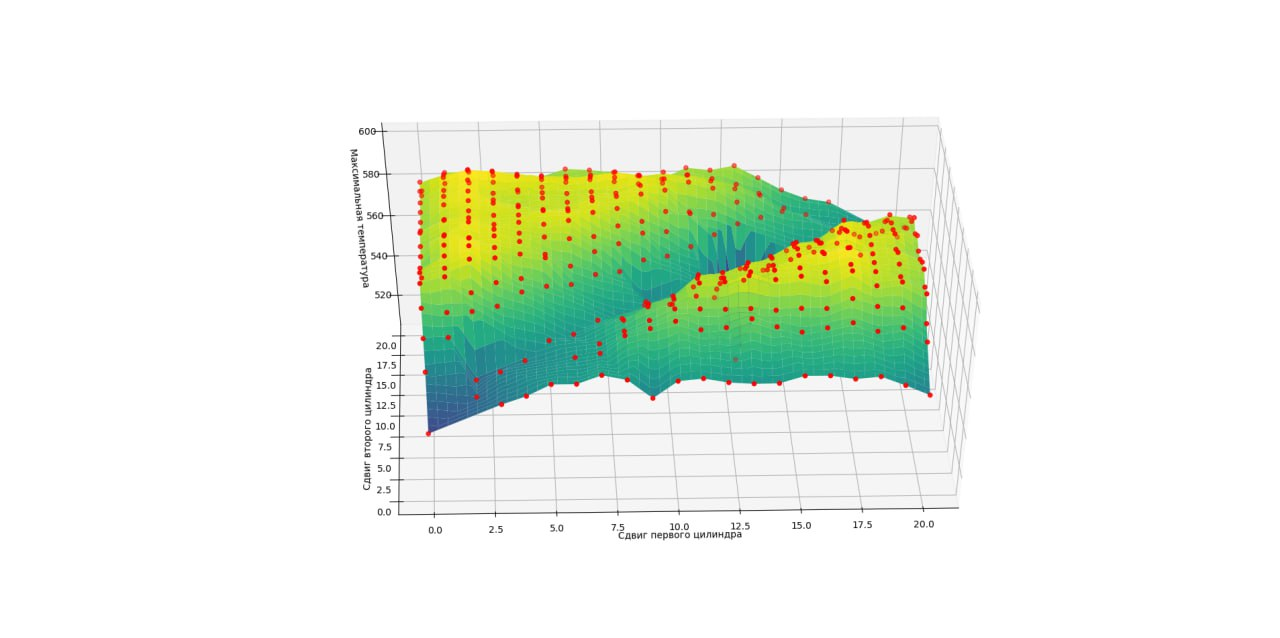
\includegraphics[width=0.4\linewidth]{18.1.jpg}
		\caption{Зависимость максимальной температуры нагревателя от сдвигов цилиндров (441 точка)} %% подпись к рисунку
	\end{center}
\end{figure}
\begin{figure}[h]
	\begin{center}
		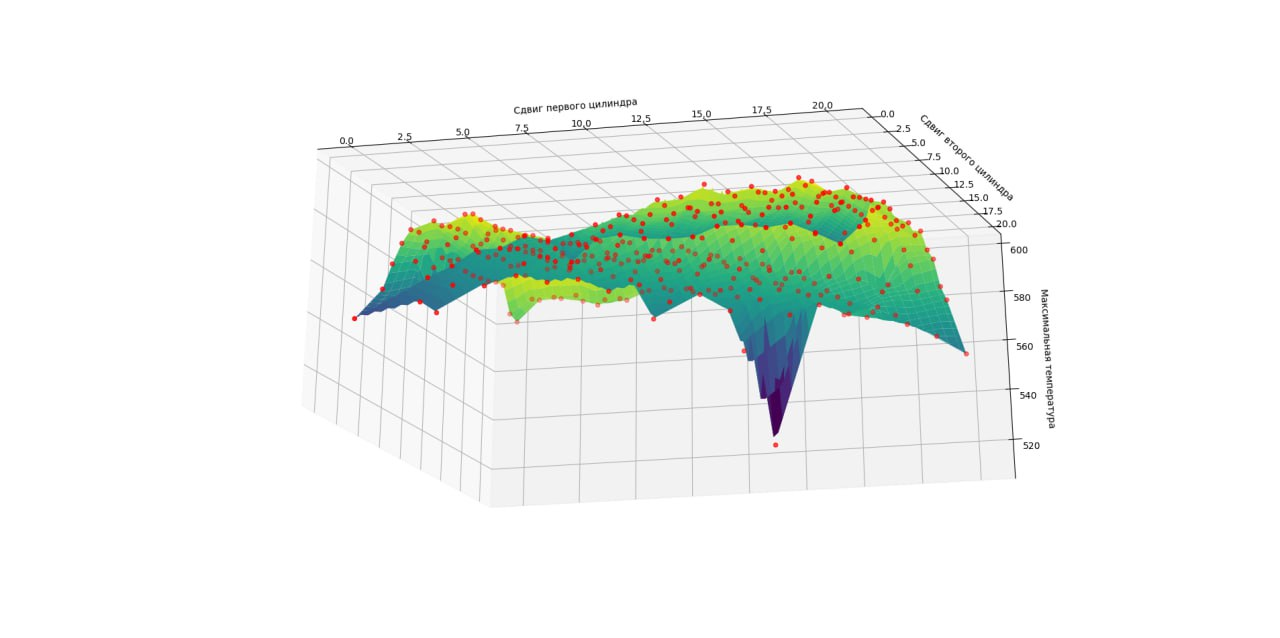
\includegraphics[width=0.4\linewidth]{18.2.jpg}
		\caption{Зависимость максимальной температуры нагревателя от сдвигов цилиндров (441 точка)} %% подпись к рисунку
	\end{center}
\end{figure}

\section{Первые результаты и наблюдения}

Первые результаты анализа геометрии системы показали интересные закономерности. В частности, было отмечено, что минимумы характеристик системы наблюдаются при равных сдвигах первого и второго цилиндров.

\begin{figure}[h]
	\begin{center}
		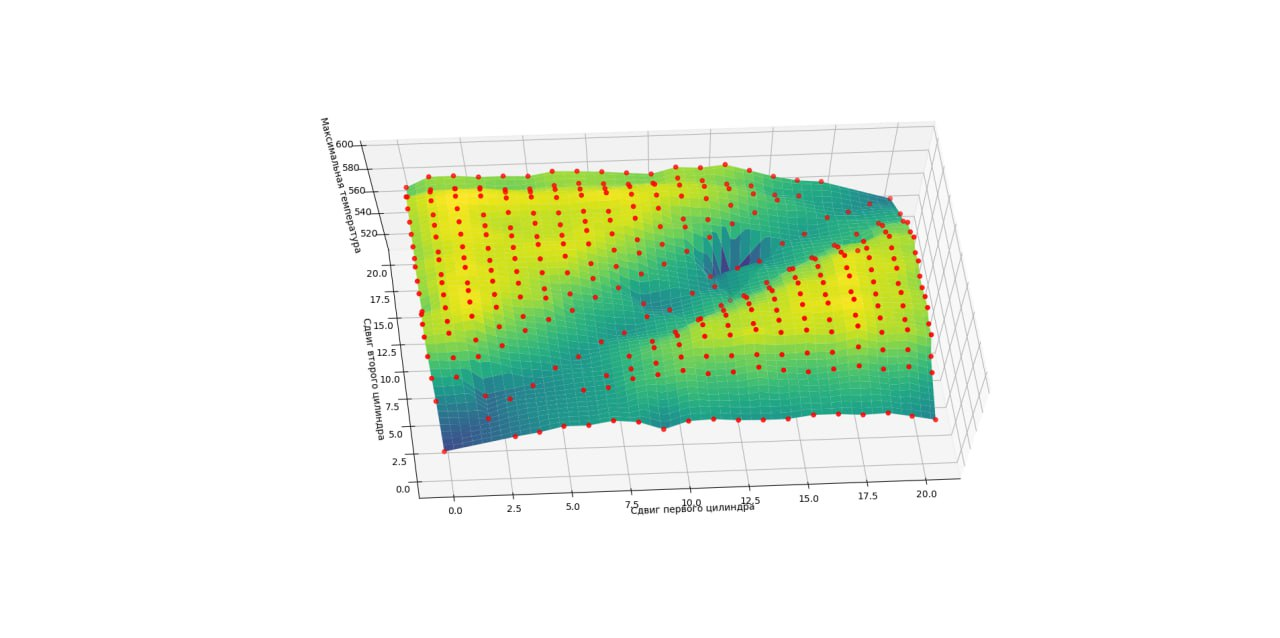
\includegraphics[width=0.4\linewidth]{18.3.jpg}
		\caption{Зависимость максимальной температуры нагревателя от сдвигов цилиндров (441 точка)} %% подпись к рисунку
	\end{center}
\end{figure}

При равных сдвигах цилиндров они касаются друг друга. Такая конфигурация способствует более эффективному теплообмену между цилиндрами и более равномерному распределению тепловой нагрузки.

\begin{figure}[h]
	\begin{center}
		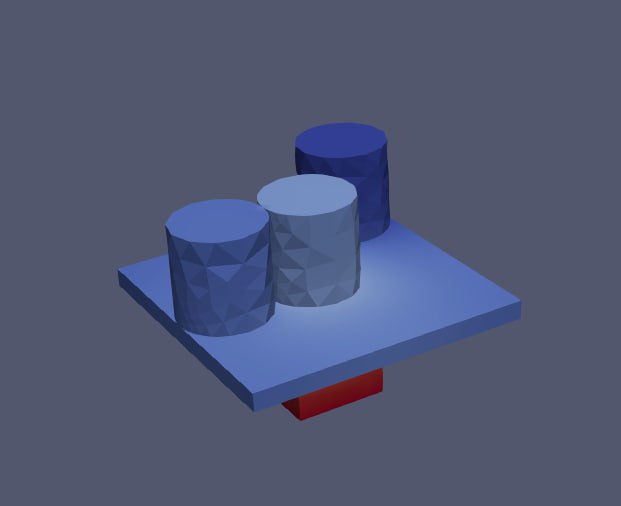
\includegraphics[width=0.4\linewidth]{19.jpg}
		\caption{Геометрия при которой достигается минимальное значение} %% подпись к рисунку
	\end{center}
\end{figure}

\section{Эксперименты с геометрией и анализ результатов}

Однако эта геометрия не демонстрировала реальной зависимости между расположением цилиндров и температурой. В ответ на это наблюдение был проведен ряд экспериментов с общей геометрией системы.

В первом эксперименте было решено уменьшить диаметр цилиндров в два раза, сделав их тоньше (2.5 мм). Это привело к тому, что цилиндры перестали касаться друг друга, создавая новые условия для теплообмена. Теперь теплообмен между цилиндрами осуществляется через воздушный зазор.

\begin{figure}[h]
	\begin{center}
		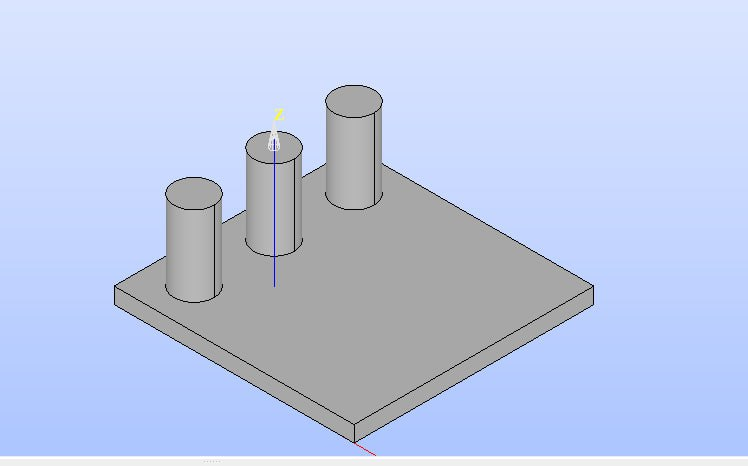
\includegraphics[width=0.4\linewidth]{20.jpg}
		\caption{Новая геометрия} %% подпись к рисунку
	\end{center}
\end{figure}

После внесения изменений в геометрию системы были получены более интересные результаты, которые отличаются от предыдущих экспериментов. Новая конфигурация цилиндров более чувствительна к расположению внутри системы, и температурные различия стали более заметными.

Например, можно заметить, что при размещении ближе к центру системы температуры становятся меньше. Это может быть обусловлено более равномерным распределением тепла в системе и более эффективным теплообменом.

\begin{figure}[h]
	\begin{center}
		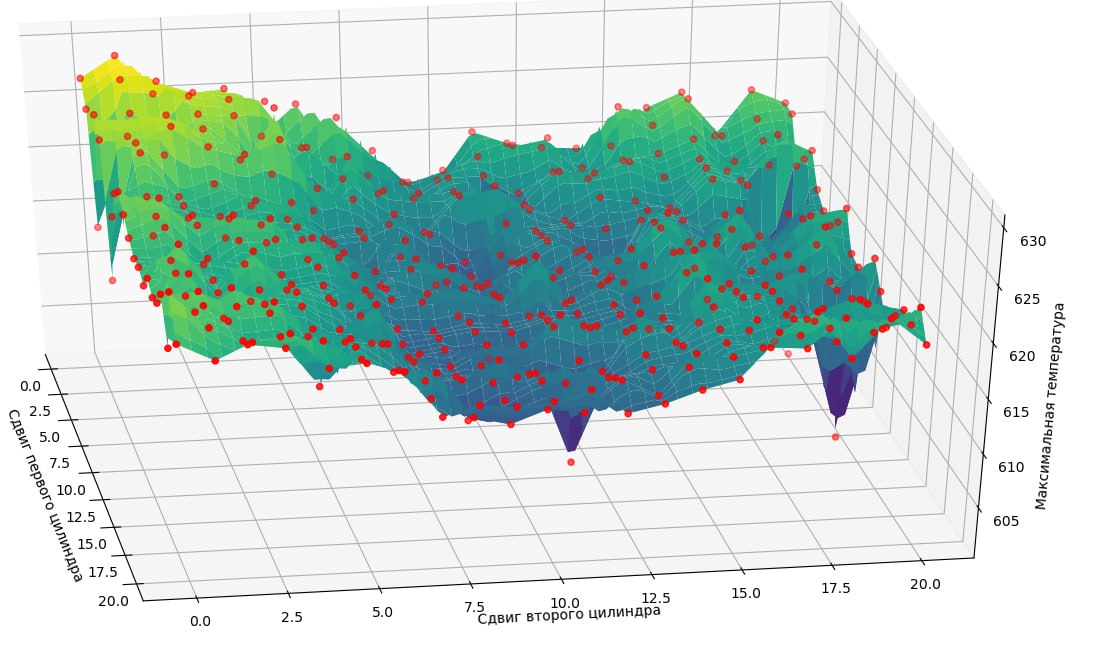
\includegraphics[width=0.4\linewidth]{21.1.jpg}
		\caption{Зависимость максимальной температуры нагревателя от сдвигов цилиндров} %% подпись к рисунку
	\end{center}
\end{figure}
\begin{figure}[h]
	\begin{center}
		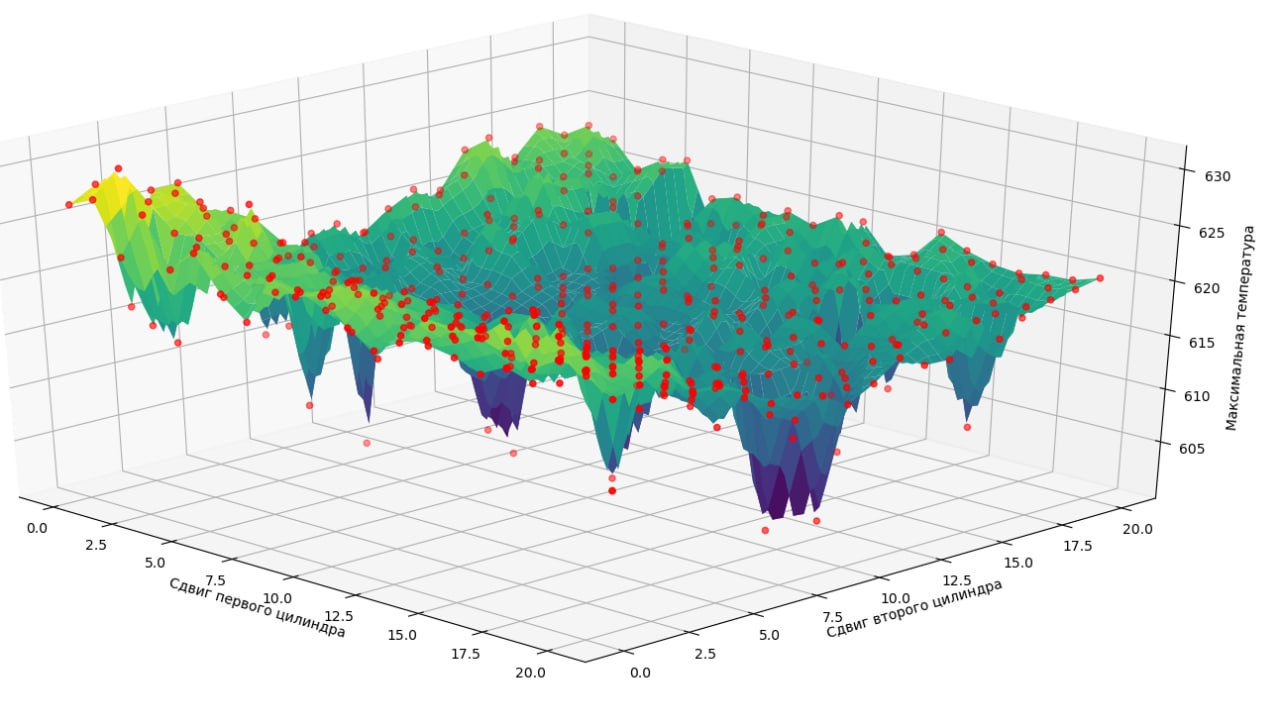
\includegraphics[width=0.4\linewidth]{21.2.jpg}
		\caption{Зависимость максимальной температуры нагревателя от сдвигов цилиндров} %% подпись к рисунку
	\end{center}
\end{figure}
\begin{figure}[h]
	\begin{center}
		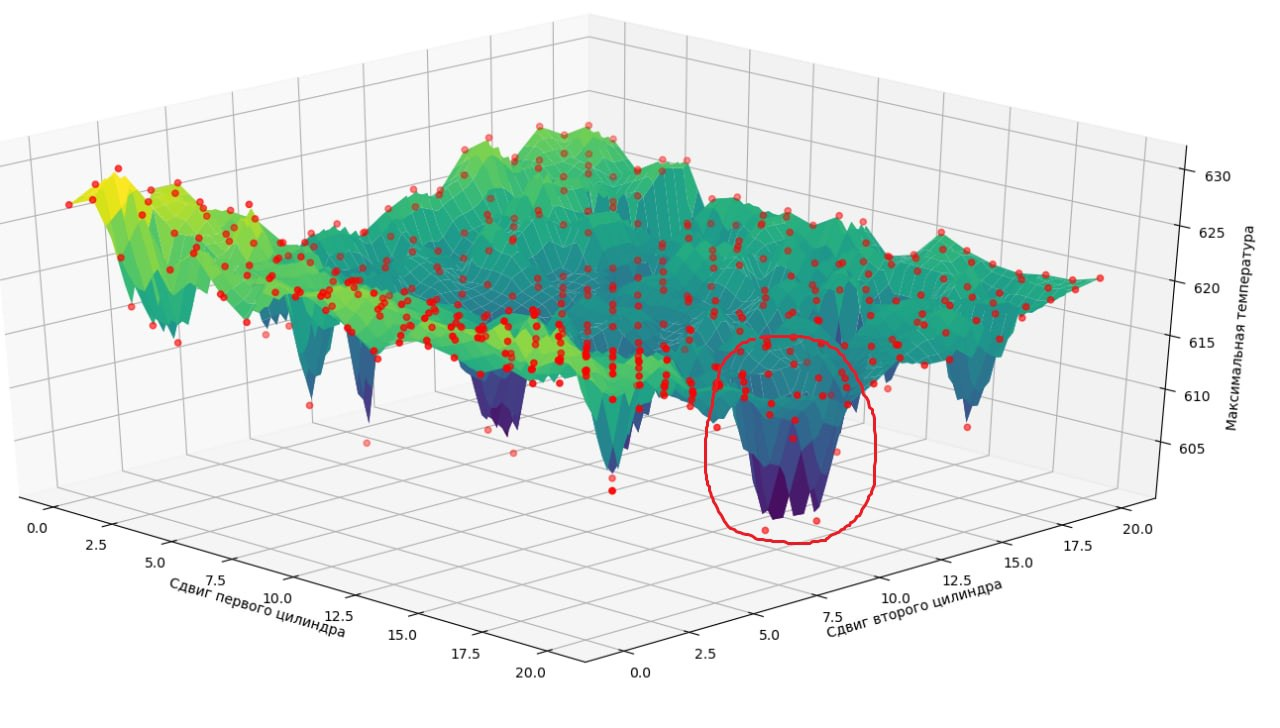
\includegraphics[width=0.4\linewidth]{21.3.jpg}
		\caption{Зависимость максимальной температуры нагревателя от сдвигов цилиндров} %% подпись к рисунку
	\end{center}
\end{figure}

В ходе экспериментов было обнаружено, что существует оптимальная конфигурация, при которой достигается минимум температуры в системе. Эта конфигурация характеризуется расстановкой цилиндров по диагонали.

\begin{figure}[h]
	\begin{center}
		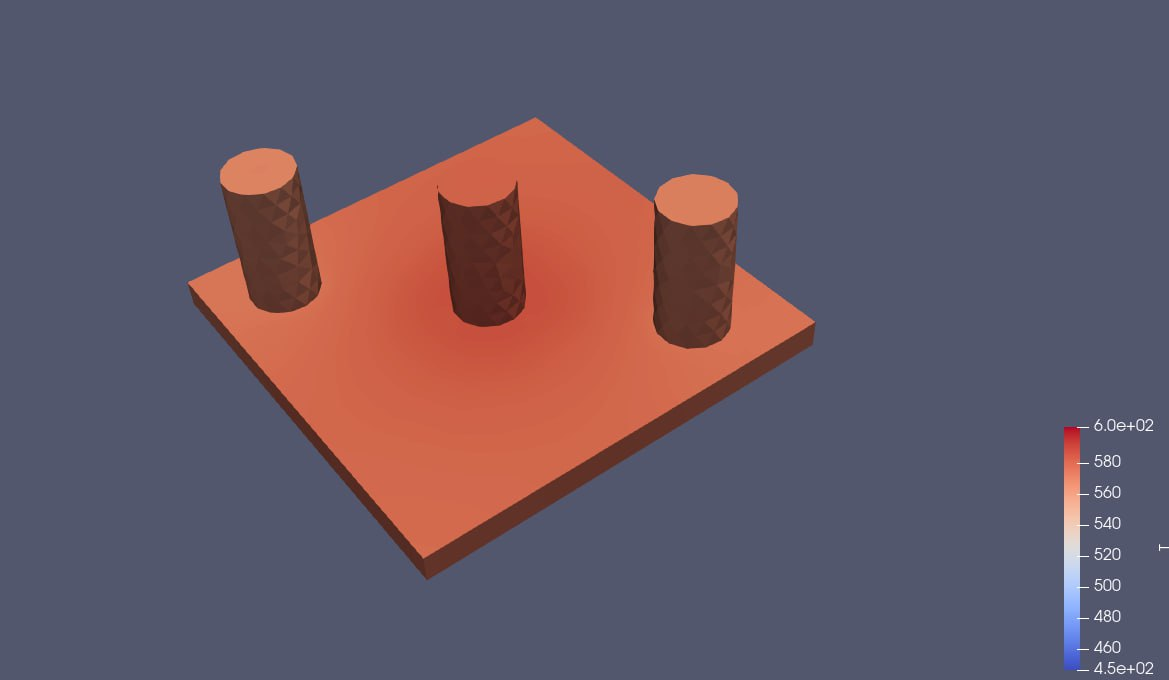
\includegraphics[width=0.4\linewidth]{21.4.jpg}
		\caption{Пример миниму при новой геометрии} %% подпись к рисунку
	\end{center}
\end{figure}

\newpage
А также при данной конфигурации будет достигаться минимум максимальной температуры нагревателя.

\begin{figure}[h]
	\begin{center}
		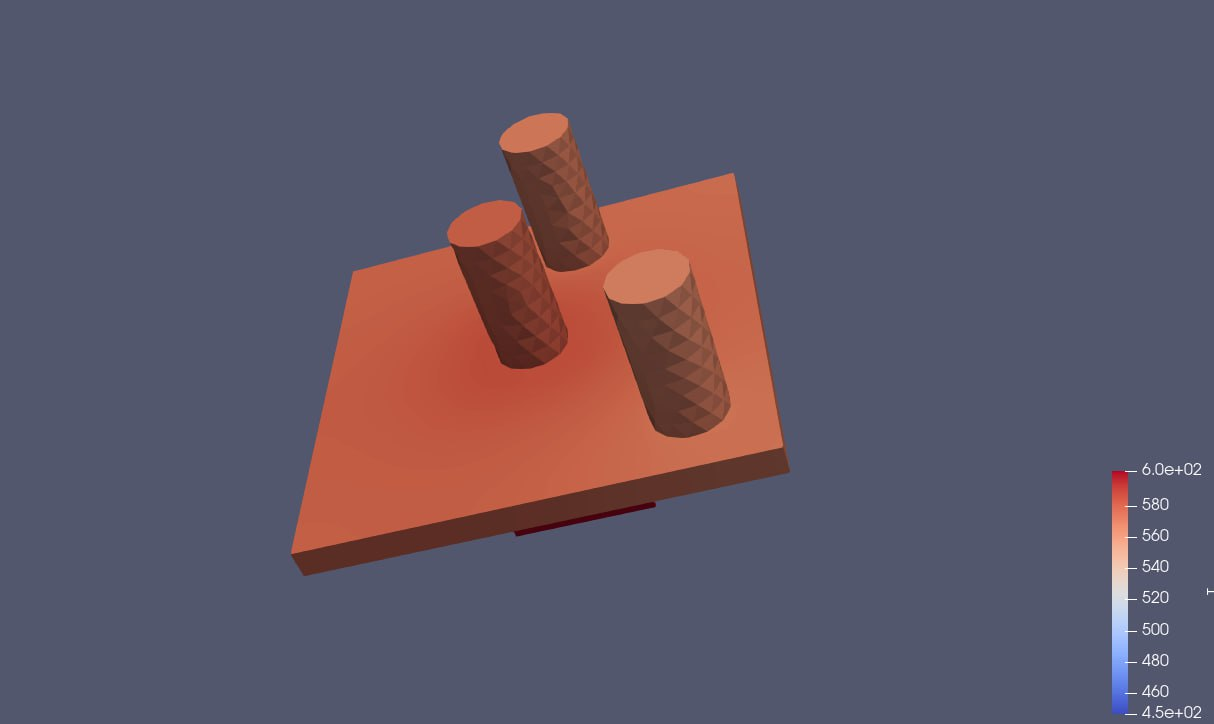
\includegraphics[width=0.4\linewidth]{21.5.jpg}
		\caption{Пример минимума при новой геометрии} %% подпись к рисунку
	\end{center}
\end{figure}

\section{Оптимизация расчетной сетки}

Для более глубокого анализа системы и выявления потенциальных выбросов в температурных данных, мы решили оптимизировать расчетную сетку. Используя параметры NETGEN\_3D, мы уменьшили размер элементов сетки.

Этот подход позволил нам более детально рассмотреть поведение системы в местах с высокими градиентами температуры и выделить потенциальные выбросы. Результаты показали, что некоторые точки действительно являются выбросами, что может быть связано с особенностями теплового распределения в этих областях.

\section{Модификация геометрии и уменьшение воздуховода}

Далее мы провели серию изменений в геометрии системы. Одним из ключевых моментов было уменьшение воздуховода практически до минимального зазора в 2 мм к цилиндрам. Это решение позволило избежать дополнительных условий на границе между воздуховодом и цилиндрами, создавая более естественные условия для теплового обмена.

С учетом внесенных изменений в геометрию системы и уменьшения воздуховода, мы провели новый ряд расчетов и получили следующие результаты.

\begin{figure}[h]
	\begin{center}
		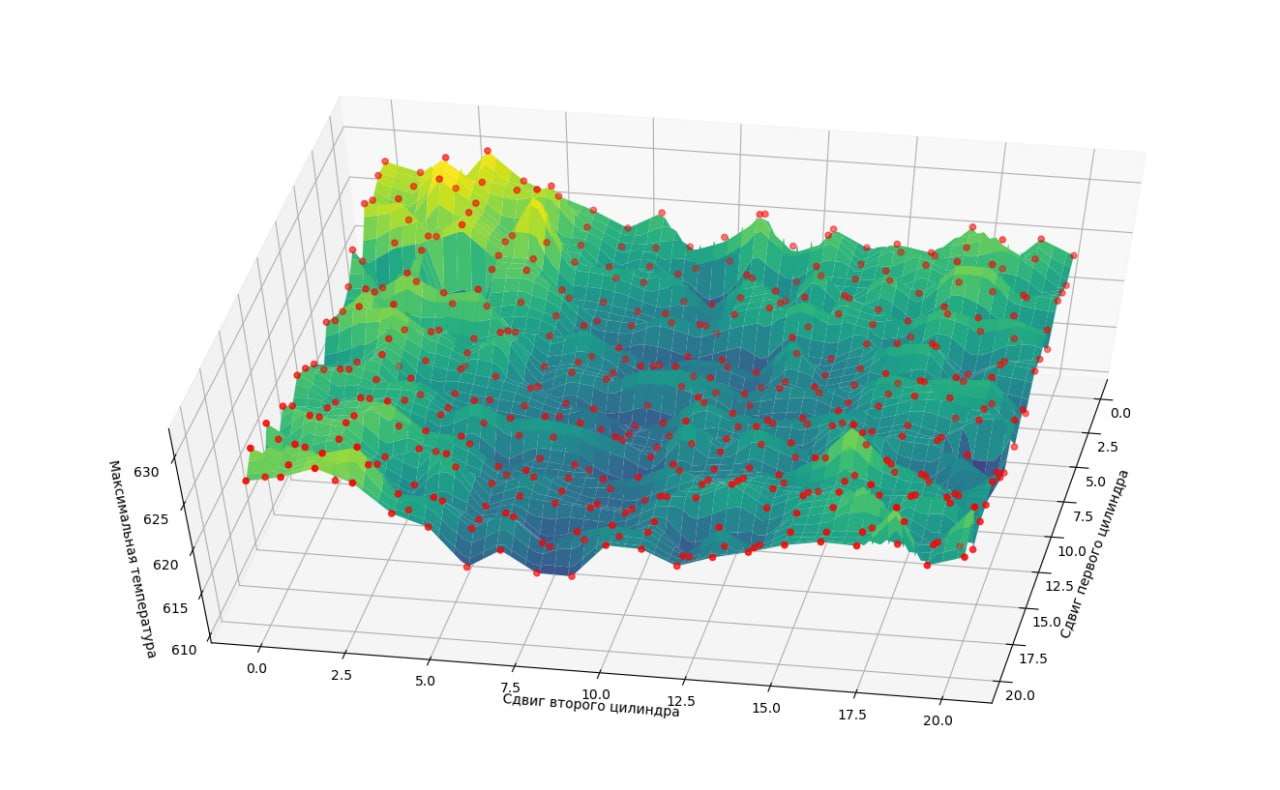
\includegraphics[width=0.4\linewidth]{22.1.jpg}
		\caption{Зависимость максимальной температуры нагревателя от сдвигов цилиндров} %% подпись к рисунку
	\end{center}
\end{figure}
\begin{figure}[h]
	\begin{center}
		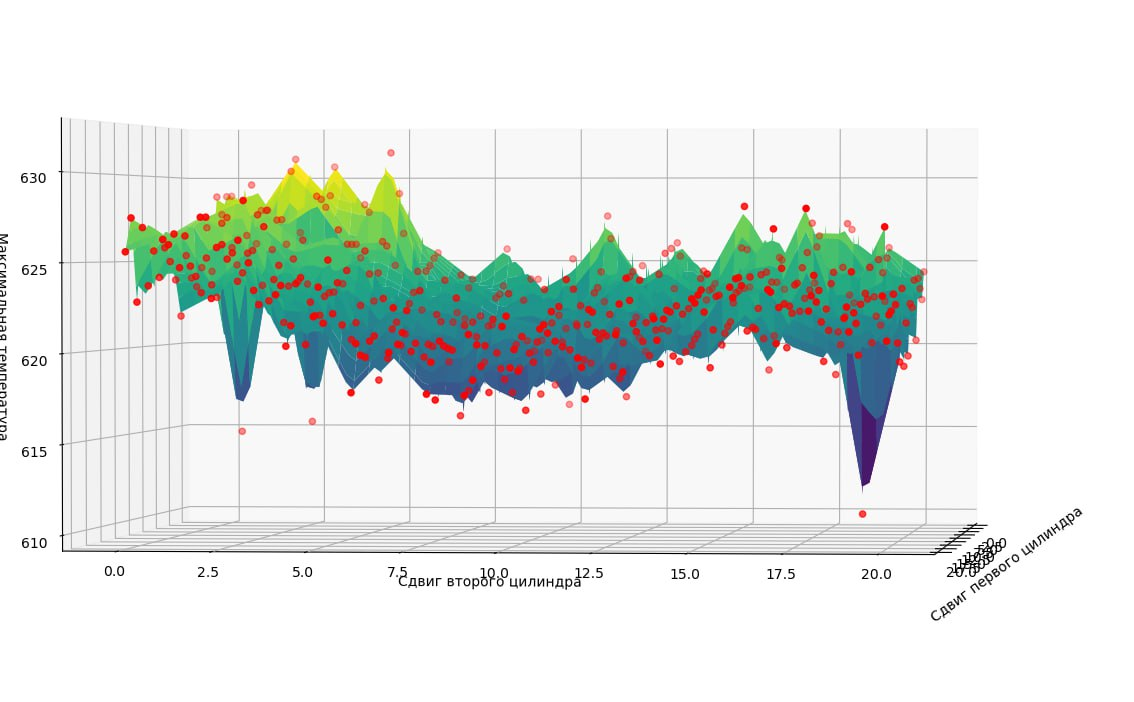
\includegraphics[width=0.4\linewidth]{22.2.jpg}
		\caption{Зависимость максимальной температуры нагревателя от сдвигов цилиндров} %% подпись к рисунку
	\end{center}
\end{figure}
\begin{figure}[h]
	\begin{center}
		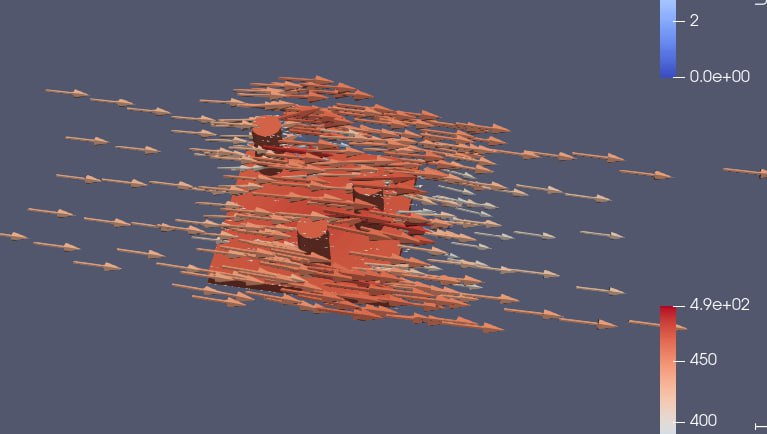
\includegraphics[width=0.4\linewidth]{22.3.jpg}
		\caption{Скорость течения} %% подпись к рисунку
	\end{center}
\end{figure}
\begin{figure}[h]
	\begin{center}
		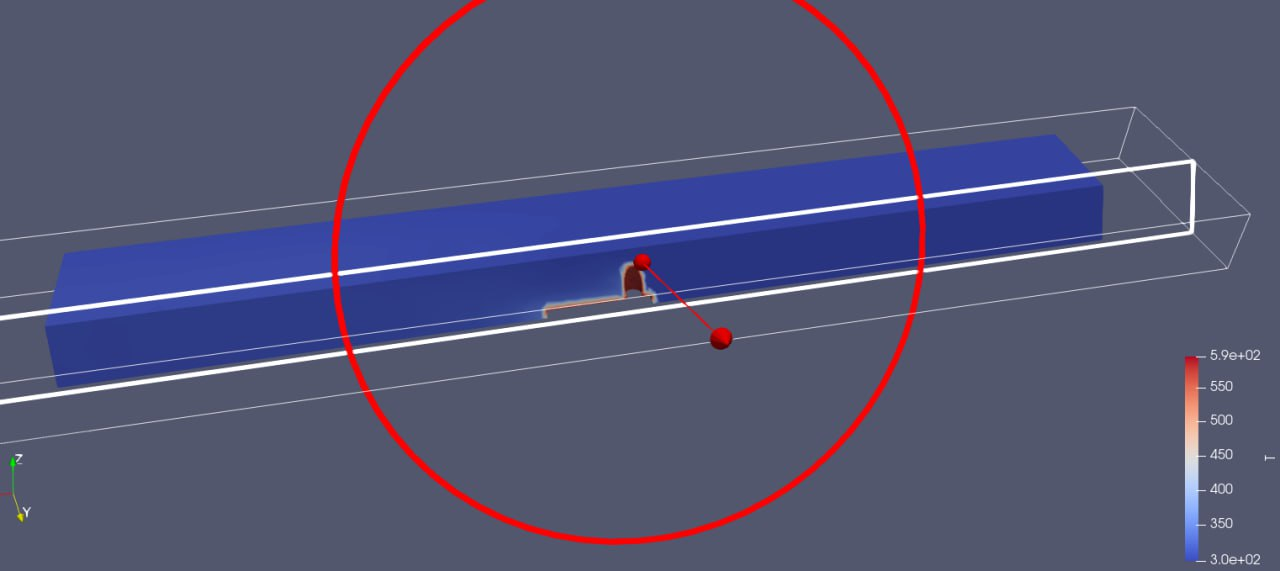
\includegraphics[width=0.4\linewidth]{22.4.jpg}
		\caption{Новая геометрия} %% подпись к рисунку
	\end{center}
\end{figure}

\section{Анализ реальной системы и изменения параметров}

Далее в нашем исследовании мы перешли к анализу более реалистичных условий, представляющих реальную систему охлаждения. Внесенные изменения включают снижение скорости воздуха внутри воздуховода до 3 м/с (по сравнению с предыдущим значением 5.6 м/с), замену материала радиатора на медь (предыдущий материал - алюминий), а также модификацию геометрии нагревателя, сделав его тоньше и значительно больше по размерам, а саму подложку радиатора сделав толще.

\begin{figure}[h]
	\begin{center}
		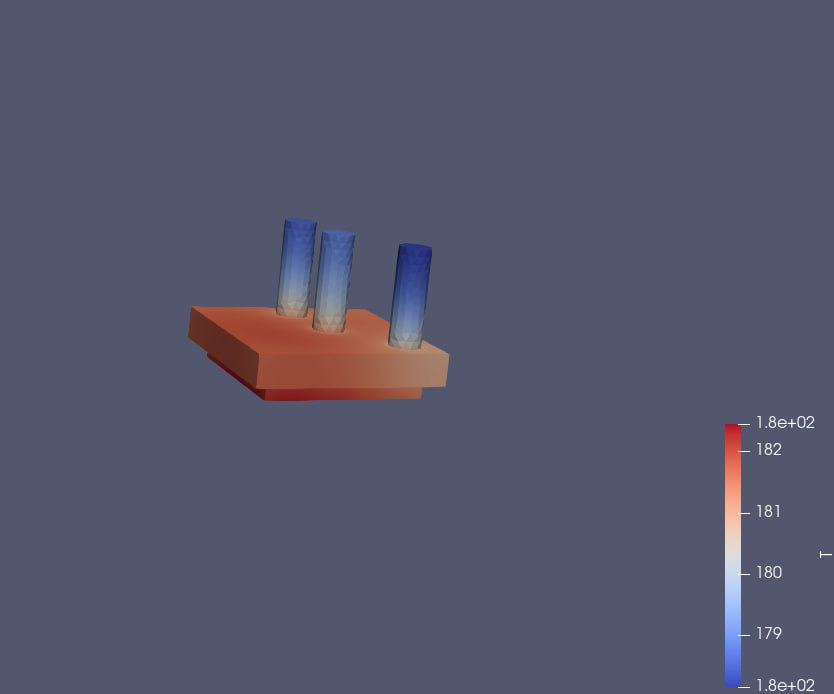
\includegraphics[width=0.4\linewidth]{23.1.jpg}
		\caption{Измененная геометрия} %% подпись к рисунку
	\end{center}
\end{figure}
\begin{figure}[h]
	\begin{center}
		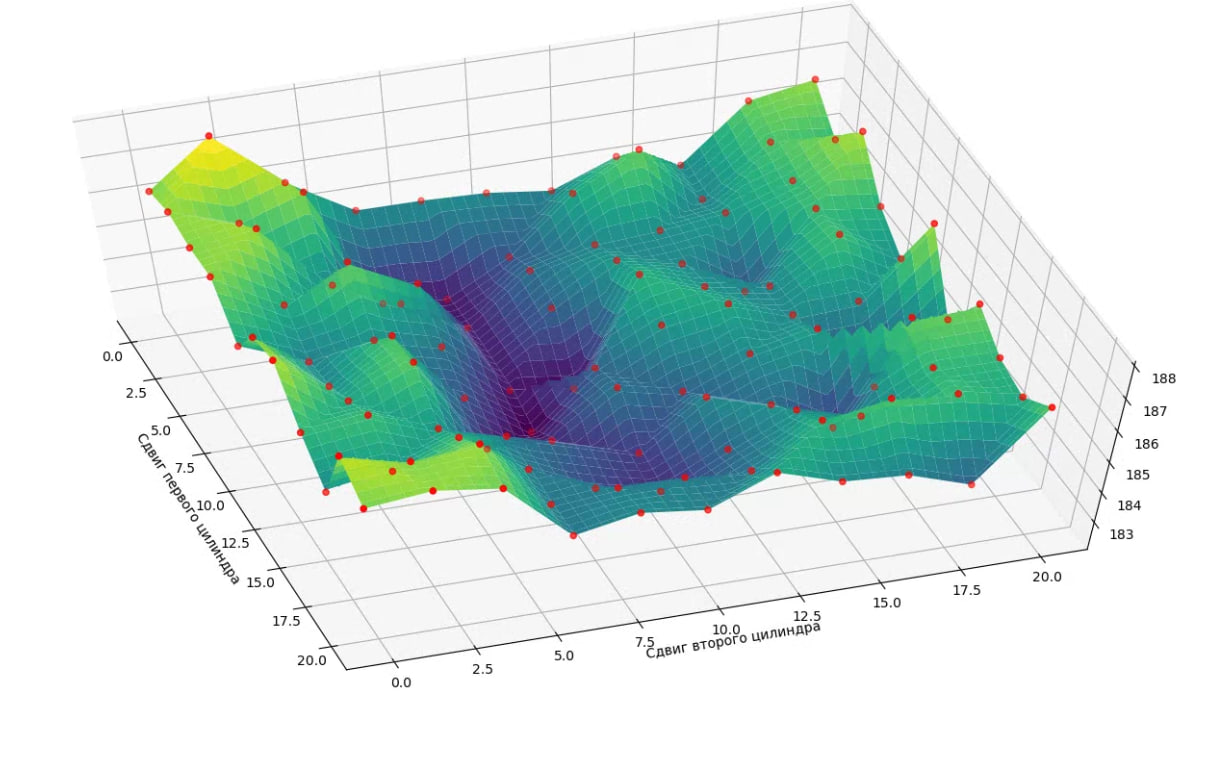
\includegraphics[width=0.4\linewidth]{23.2.jpg}
		\caption{Зависимость максимальной температуры нагревателя от сдвигов цилиндров} %% подпись к рисунку
	\end{center}
\end{figure}
\begin{figure}[h]
	\begin{center}
		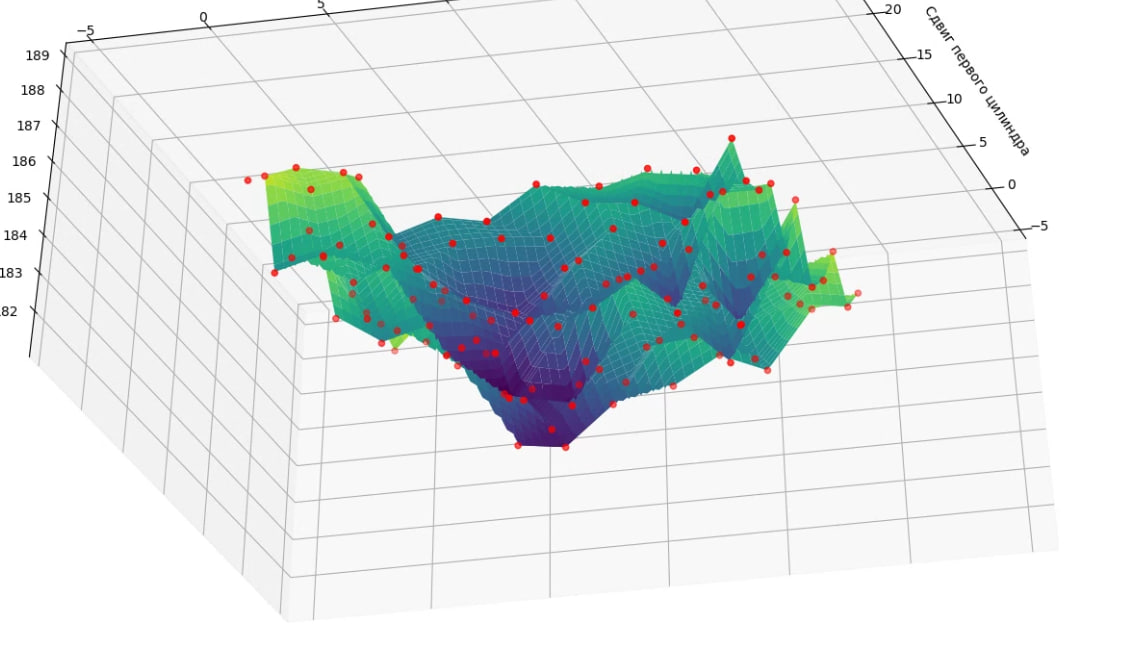
\includegraphics[width=0.4\linewidth]{23.3.jpg}
		\caption{Зависимость максимальной температуры нагревателя от сдвигов цилиндров} %% подпись к рисунку
	\end{center}
\end{figure}

\section{Применение эволюционного алгоритма в оптимизации}

Для более эффективного и быстрого поиска оптимальных параметров в задаче охлаждения был применен эволюционный алгоритм. Эволюционные алгоритмы — это класс методов оптимизации, вдохновленных процессами биологической эволюции. Они включают в себя механизмы отбора, скрещивания и мутации, а применительно к задачам оптимизации, такие алгоритмы позволяют находить оптимальные решения в пространствах больших размерностей.

Принцип работы эволюционного алгоритма можно кратко описать следующим образом:

\begin{enumerate}
    \item \textbf{Инициализация популяции:} Создается начальная популяция индивидов (наборов параметров) случайным образом или на основе каких-то эвристик.

    \item \textbf{Оценка приспособленности:} Каждый индивид из популяции оценивается по степени приспособленности в соответствии с целевой функцией. В нашем контексте целевая функция - минимизация максимальной температуры внутри нагревателя.

    \item \textbf{Отбор:} Выбираются наиболее приспособленные индивиды для следующего поколения. Это может происходить различными методами, такими как турнирный отбор, рулеточный отбор и др.

    \item \textbf{Скрещивание:} Происходит кроссовер (скрещивание) между выбранными индивидами, что приводит к созданию новых индивидов. Это позволяет объединить положительные черты родителей.

    \item \textbf{Мутация:} Некоторые индивиды могут подвергаться мутациям, изменяя свои параметры с определенной вероятностью. Это вносит элемент случайности и разнообразия в популяцию.

    \item \textbf{Повторение:} Описанные шаги повторяются в цикле до достижения критерия остановки, такого как заданное количество поколений или достижение требуемой точности.
\end{enumerate}

Эволюционные алгоритмы являются мощным инструментом для оптимизации в больших пространствах параметров, позволяя находить приближенно оптимальные решения в условиях ограниченной информации о системе.

Применение эволюционного алгоритма в задаче оптимизации параметров системы охлаждения значительно снизило количество необходимых расчетов. Вместо полного перебора всех 441 точек в пространстве параметров, алгоритм смог достичь точек минимума всего за 50 расчетов.

\section{Использование градиентного метода}

Помимо дифференциальной эволюции, наша работа включала использование градиентного метода для оптимизации. Градиентные методы основаны на использовании градиента (производной) целевой функции для нахождения экстремума. В контексте оптимизации, где целью является минимизация или максимизация функции, градиентный метод может эффективно приближаться к оптимальному решению.

В рамках градиентного метода особенно полезными являются методы оптимизации с использованием градиента первого и второго порядка, такие как метод наименьших квадратов (L-BFGS-B) или метод сопряженных градиентов (CG).

Преимущества использования градиентных методов включают:

\begin{enumerate}
    \item \textbf{Быстрая сходимость:} Градиентные методы могут сходиться быстро, особенно при правильном выборе параметров и хорошей обусловленности задачи.

    \item \textbf{Точность результатов:} Градиентные методы могут предоставить точные результаты в задачах, где необходимо достичь высокой точности оптимизации.
\end{enumerate}

\begin{figure}[h]
	\begin{center}
		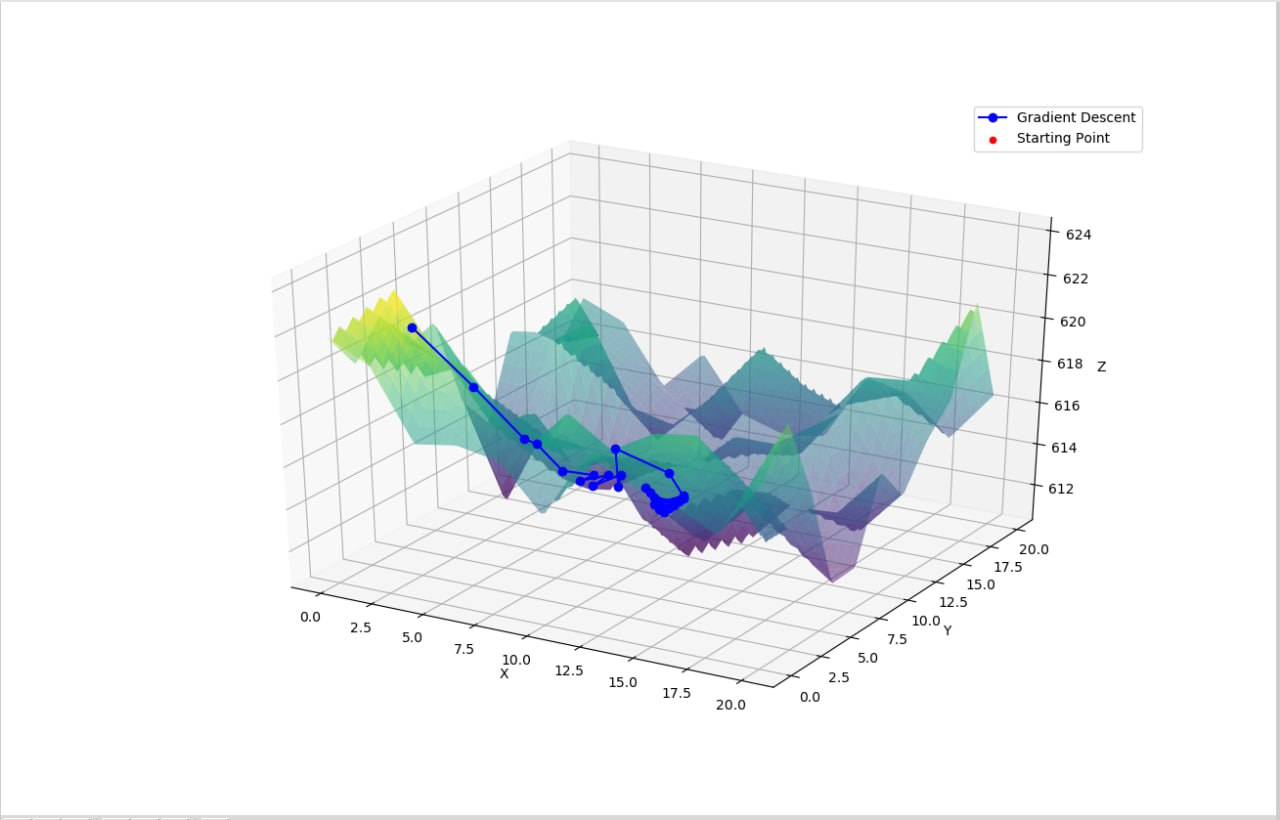
\includegraphics[width=0.4\linewidth]{24.jpg}
		\caption{Зависимость максимальной температуры нагревателя от сдвигов цилиндров} %% подпись к рисунку
	\end{center}
\end{figure}

\newpage
\section{Заключение}

В ходе нашей работы мы провели комплексное исследование системы охлаждения, используя численные методы и оптимизацию. Ниже представлены ключевые выводы и результаты нашей работы:

\begin{enumerate}
    \item \textbf{Геометрические изменения:} Изначально мы провели анализ геометрии системы, исследуя влияние расположения цилиндров на эффективность охлаждения. Эксперименты с различными конфигурациями позволили нам выявить оптимальные расстановки и влияние контакта цилиндров друг с другом на тепловые характеристики.

    \item \textbf{Оптимизация с использованием полного перебора:} Мы провели первоначальную оптимизацию системы, используя полный перебор, что позволило нам выявить оптимальные точки в пространстве параметров. Это дало общий обзор зависимостей и минимумов целевой функции.

    \item \textbf{Многопоточность для улучшения производительности:} В процессе увеличения количества точек в пространстве параметров мы использовали многопоточность для оптимизации, что значительно ускорило процесс расчета и позволило нам провести более подробное исследование.

    \item \textbf{Изменения в геометрии и параметрах системы:} Мы исследовали влияние различных параметров, таких как скорость воздуха и материалы, на эффективность охлаждения. Изменения в геометрии и параметрах системы привели к новым интересным результатам, позволяя лучше понять зависимости и оптимизировать систему.

    \item \textbf{Эволюционный алгоритм:} Мы применили эволюционный алгоритм для оптимизации системы. Этот метод позволил нам более эффективно находить точки минимума, снижая количество расчетов по сравнению с полным перебором.

    \item \textbf{Градиентные методы оптимизации:} Использование градиентных методов, таких как L-BFGS-B, добавило эффективность и точность в наш арсенал оптимизационных методов.

    \item \textbf{Выводы и перспективы:} На основе результатов исследования мы делаем вывод о том, что оптимизация геометрии и параметров системы охлаждения может существенно повысить ее эффективность. Подход с использованием различных методов оптимизации и численного моделирования предоставляет мощный инструментарий для разработки и улучшения теплоотводящих систем. В будущем возможно проведение более глубоких исследований с учетом дополнительных факторов и условий эксплуатации системы.
\end{enumerate}

\newpage
\bibliographystyle{utf8gost705u}  %% стилевой файл для оформления по ГОСТу
\bibliography{Overview}     %% имя библиографической базы (bib-файла) 

\newpage
\section{Приложение А}
% \renewcommand{\thesection}{\Asbuk{section}}
Проект можно найти на github (github.com/AlexEsn/FOAM\_project), где содержатся все скрипты и кейсы.

\newpage
\section{Приложение Б}
% \renewcommand{\thesection}{\Asbuk{section}}
В процессе работы был найден баг в SALOME-9.9.0: при дампе Python скрипта с сеткой создается файл с ошибкой.

\begin{figure}[h]
	\begin{center}
		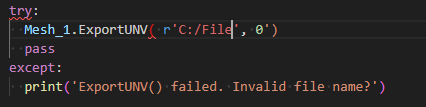
\includegraphics[width=1\linewidth]{e.png}
		\caption{Ошибка экспорта сетки} %% подпись к рисунку
	\end{center}
\end{figure}

Для её решения достаточно удалить лишние символы:
\begin{figure}[h]
	\begin{center}
		\includegraphics[width=1\linewidth]{er.png}
		\caption{Решение ошибки экспорта сетки} %% подпись к рисунку
	\end{center}
\end{figure}


\end{document}